% !TeX spellcheck = en_US
% LANGUAGE INCONSISTENCIES FOUND:
% -ise verbs found in the text.
%  LaTeX support: latex@mdpi.com

\documentclass[symmetry,article,accept,pdftex,moreauthors]{Definitions/mdpi}

% MDPI internal commands - do not modify
\firstpage{1}
\makeatletter
\setcounter{page}{\@firstpage}
\makeatother
\pubvolume{1}
\issuenum{1}
\articlenumber{0}
\pubyear{2026}
\copyrightyear{2026}
\externaleditor{Firstname Lastname} % More than 1 editor, please add `` and '' before the last editor name
\datereceived{11 May 2026}
\daterevised{8 July 2026}
\dateaccepted{9 July 2026}
\datepublished{ }
%Author general note: Please replace the placeholder editor name, volume, issue, article number, publication date, and DOI with the final production metadata before publication. We have not modified the MDPI internal commands.

\Title{Multi-Granularity Feature Decomposition with Ranking-Aware Regularization for Old Film Restoration}

%\input{sections/authors}
% Author information for MGFROFR paper
% MDPI Symmetry format
% This file is input by MGFROFR.tex.

\newcommand{\orcidauthorA}{0009-0000-1111-7667}
\newcommand{\orcidauthorB}{0009-0008-9432-7018}

\Author{\hl{Feifan} Cai %MDPI: Please carefully check the accuracy of names and affiliations.
%Author: We carefully checked and confirm that the author names, author order, and affiliations are correct as shown.
 $^{1,2,3}$\orcidA{}, Qi \hl{Zhang} $^{1,2}$\highlighting{\orcidB{},} %MDPI: we detected the ORCID 0000-0002-3827-1522 didn't match the author name Qi Zhang, so we removed it, please check and confirm.
%Author: Corrected; the ORCID for Qi Zhang has been updated to the verified matching iD (\orcidauthorB).
 Kun Yang $^{3}$, Lei Chen $^{3}$ and Youdong Ding $^{1,2,}$*}

\AuthorNames{Feifan Cai, Qi Zhang, Kun Yang, Lei Chen and Youdong Ding}

\address{%
$^{1}$ \quad Shanghai Film Academy, Shanghai University, 788 Guangzhong Road, Shanghai 200072, China;  \hl{feifan@shu.edu.cn (F.C.); zq10501@shu.edu.cn (Q.Z.)} %MDPI: We added these email addresses here according to those submitted online at susy.mdpi.com. Please confirm. The following highlights are the same.
%Author: We confirm that the added email addresses are correct: feifan@shu.edu.cn (F.C.), zq10501@shu.edu.cn (Q.Z.), yangkun@tyut.edu.cn (K.Y.), and chenlei839@163.com (L.C.).
\\
$^{2}$ \quad Shanghai Engineering Research Center of Motion Picture Special Effects, Shanghai 200072, China\\
$^{3}$ \quad College of Mechanical Engineering, Taiyuan University of Technology, Taiyuan 030024, China; \hl{yangkun@tyut.edu.cn (K.Y.); chenlei839@163.com (L.C.)}}

\corres{Correspondence: ydding@shu.edu.cn}
%\input{sections/abstract}
\abstract{\highlighting{Old} %MDPI: Please define all abbreviations when they first appear in the abstract, main text, and figure or table captions.
%Author: We audited abbreviations independently in the abstract, main text, and figure/table scope and defined them at first use in each scope. The abstract defines MgfrOFR and SRWOV; the main text now defines the method, module, metric, hardware/software, and dataset abbreviations used there; and the relevant figure/table captions define their own first-use abbreviations, including DCN, ROI, GT, MAE, the full-reference and no-reference metrics, the method acronyms in the first comparison table, FLOPs, and FPS. We also corrected REDS to "REalistic and Dynamic Scenes", explained "Concat" in the first architecture figure, and updated the key Abbreviations list to match the rendered manuscript.
 film restoration remains challenging because archival footage often combines scratches, blotches, flicker, blur, and temporal artifacts, disrupting the balance among structural recovery, regional texture repair, and fine artifact suppression. We propose Multi-Granularity Feature Decomposition with Ranking-Aware Regularization for Old Film Restoration (MgfrOFR), a multi-granularity extension of a Mamba-based old film restoration backbone. MgfrOFR first decomposes propagated features into coarse-to-fine restoration branches and feeds branch summaries back through channel-wise recalibration so different degradation scales can be represented without competing in a single feature stream. It then introduces a ranking-aware triplet regularizer that penalizes correlated temporal-similarity rankings across branches during training while preserving the baseline inference interface. Experiments on the Synthetic/Real-World Old Video (SRWOV) benchmark show statistically significant fidelity gains on synthetic clips, favorable no-reference naturalness on real-world archival footage, and a bounded perceptual-quality trade-off. These results indicate that representation-level branch balance is an effective inductive bias for old film restoration under heterogeneous and asymmetric~degradation.}

\keyword{old film restoration; multi-granularity feature decomposition; ranking-aware regularization; state space models; feature space symmetry}

\usepackage{algorithm}
\usepackage{algpseudocode}
\usepackage{placeins}
\DeclareRobustCommand{\bestres}[1]{\textcolor{red}{#1}}
\DeclareRobustCommand{\secondres}[1]{\textcolor{blue}{#1}}
\renewcommand{\topfraction}{0.9}
\renewcommand{\bottomfraction}{0.8}
\renewcommand{\textfraction}{0.08}
\renewcommand{\floatpagefraction}{0.85}
\setlength{\textfloatsep}{10pt plus 2pt minus 2pt}
\setlength{\floatsep}{8pt plus 2pt minus 2pt}
\setlength{\intextsep}{8pt plus 2pt minus 2pt}
\setlength{\headheight}{20pt}

% Reduce widow/orphan penalties to prevent large blank areas caused by
% MDPI's strict default (10000). 300 still discourages widows/clubs
% but allows LaTeX to break paragraphs when a page has remaining space.
\clubpenalty=300
\widowpenalty=300
\displaywidowpenalty=300

% On float pages (pages that contain only floats), LaTeX vertically centers
% the content by default. Set top/bottom glue to 0 so floats stack at the
% top, eliminating the large blank areas above figures on dedicated float pages.
\makeatletter
\setlength{\@fptop}{0pt}
\setlength{\@fpbot}{0pt}
\makeatother

\AtBeginDocument{\hypersetup{
  pdftitle={Multi-Granularity Feature Decomposition with Ranking-Aware Regularization for Old Film Restoration},
  pdfsubject={Representation-level symmetry-aware multi-granularity feature balancing for old film restoration},
  pdfauthor={Feifan Cai; Qi Zhang; Kun Yang; Lei Chen; Youdong Ding},
  pdfkeywords={old film restoration, symmetry-aware representation learning, multi-granularity features, state space model}
}}

\begin{document}

%\input{sections/introduction}
\section{Introduction}
\label{sec:introduction}

Old films preserve cinematic heritage and historical documentary material and form large archival collections, yet the film stock that stores this material continues to decay. Digital restoration offers a practical route to revitalize such material~\cite{iizuka2019deepremaster}. A~central difficulty is that aged footage is rarely damaged in only one way. Scratches, dust, blotches, flicker, blur, grain, and~fading can accumulate within the same clip and act on very different spatial scales, from~large structural damage to thin local artifacts. This range of scales sets old film restoration apart from generic video enhancement. A~successful restoration model must keep coarse structural recovery, regional texture repair, and~fine artifact suppression in balance---a representation-level symmetry that asymmetric, heterogeneous degradation continually~disrupts.

Learning-based old film restoration has advanced through end-to-end video restoration frameworks. The recurrent transformer network (RTN) pioneered bidirectional recurrent propagation with a learnable defect mask, but~its restoration evidence still flows through a single recurrent stream~\cite{wan2022rtn}. The Recursive Recurrent Transformer Network (RRTN) added recursive transformer propagation for stronger temporal alignment, yet structural recovery and fine artifact suppression remain jointly encoded~\cite{lin2024rrtn}. MambaOFR introduced state space models to old film restoration, improving efficiency and establishing the Synthetic/Real-World Old Video (SRWOV) benchmark~\cite{mao2025mambaofr,gu2024mamba,guo2024mambair}. Even so, it routes every degradation scale through a single propagated feature pathway. These methods share a common limitation: when heterogeneous signals compete in one latent space, coarse recovery can overwrite fine evidence, and~local artifact suppression can distort global~structure.

Here, symmetry operates at the representation level rather than as an object-level shape constraint. A~symmetric representation keeps restoration evidence balanced across granularity-specific branches while maintaining consistent temporal correspondence across frames. Because~our branch-diversity objective is invariant under permutations of the granularity branches (the symmetric group $\mathcal{S}_G$), this balance is a permutation symmetry in the machine-learning sense---a standard group-symmetry principle---rather than a visible geometric one, placing our framework within symmetry-driven representation learning for image restoration. This interpretation fits old film restoration because its degradation space is hierarchical. Missing regions and large blotches require global context, grain and flicker require regional modeling, and~fine scratches or dust require local precision. Existing multi-granularity designs mainly target detection or recognition~\cite{lin2017fpn,wang2021hrnet,sun2018pcb,wang2018mgn,gu2025reidmamba}. Naive multi-branch extensions can still collapse into correlated features unless branch diversity is explicitly enforced. This gap motivates explicit granularity-separated restoration~branches.

We propose Multi-Granularity Feature Decomposition with Ranking-Aware Regularization for Old Film Restoration (MgfrOFR), which augments MambaOFR with two complementary components (Figure~\ref{fig:architecture}). The~Multi-Granularity Feature Extractor (MGFE) reorganizes propagated Mamba features into coarse-to-fine restoration branches so that structural completion, regional repair, and~fine-detail suppression are carried by dedicated descriptors instead of competing in one hidden stream. It also feeds branch summaries back into the spatial stream through channel-wise recalibration. Ranking-Aware Triplet Regularization (RATR) complements this decomposition by discouraging redundant branch behavior: it penalizes correlated rankings of temporal correspondences rather than imposing identity-label supervision, making the regularizer suited to~restoration.

Using a unified reproduction protocol on SRWOV, MgfrOFR preserves the efficient Mamba backbone of MambaOFR while adding explicit granularity control at modest overhead. The~main contributions are summarized as~follows:
\begin{enumerate}[nosep]
    \item We formulate old film restoration through representation-level symmetry under heterogeneous degradation, treating coarse structural recovery, regional texture repair, and~fine artifact suppression as complementary feature components that remain balanced despite spatial and temporal asymmetry.
    \item We design MGFE, a~multi-granularity feature decomposition for Mamba-based old film restoration that inserts learnable restoration tokens into propagated features, aggregates them into coarse-to-fine branches, and~feeds branch summaries back to the spatial stream through channel-wise recalibration.
    \item We introduce RATR, a~ranking-aware triplet regularizer that penalizes correlated temporal-similarity rankings across granularity branches using differentiable rank correlation, improving branch complementarity and reducing redundancy while preserving the original baseline inference interface.
    \item We evaluate MgfrOFR on the SRWOV synthetic and real-world benchmark; statistical tests, ablations, and~complexity analysis show improved restoration fidelity and no-reference \mbox{naturalness} at modest additional computational cost.
\end{enumerate}

\vspace{4pt}

\begin{figure}[t]
%Author general note: We changed the figures from forced placement to controlled floating placement to remove excessive proof-layout whitespace while preserving figure order and content.

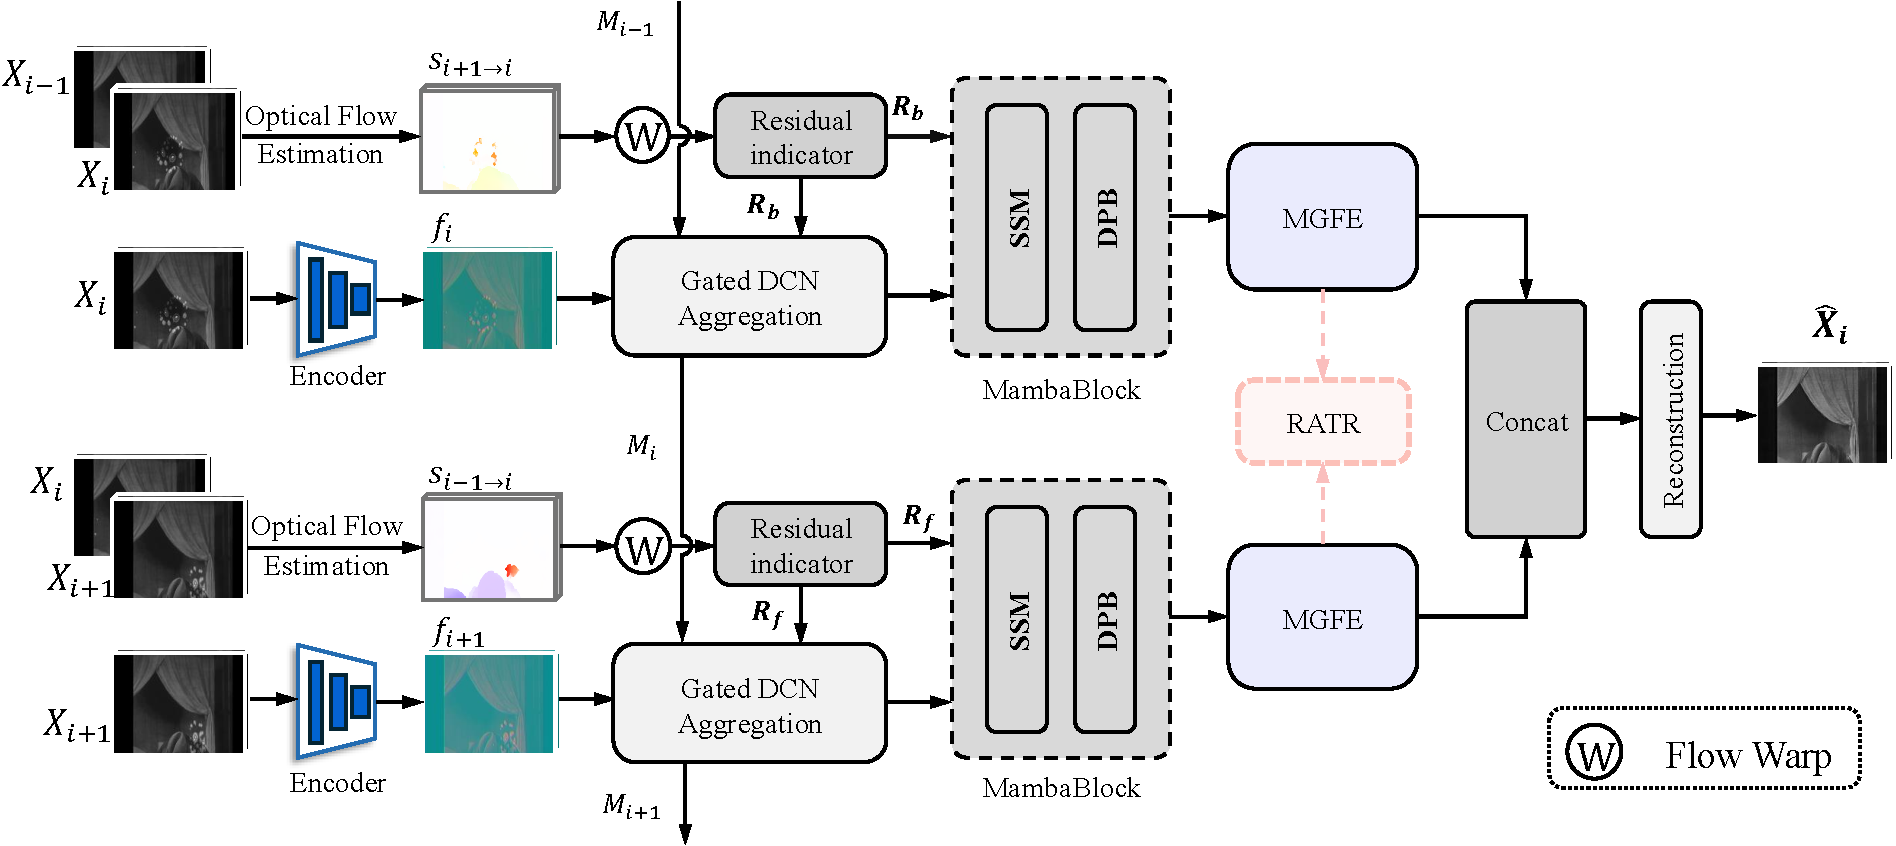
\includegraphics[width=\textwidth]{figures/Fig1_mgfrofr_architecture.pdf}
\caption{\hl{Overview} %MDPI: 1. Please note that the size/White space margin of figures will be adjusted appropriately to ensure the clarity and readability of the image, Changes to the position of figures and tables may occur during the production stage. 2. Please double check all figures, if there are special color/special symbol... need add explanation in the figure caption.
%Author: We checked all figures and added the necessary caption explanations. In Figure 1, solid black arrows denote the inference-time restoration path, light-red dashed arrows denote the training-only RATR connections, and dashed black boxes group the state space model and degradation-aware prompt block units into each MambaBlock. We also changed the figures from fixed placement to controlled floating placement to remove excessive proof-page white space; the figure content, resolution, captions, numbering, and order are unchanged. We acknowledge that figure and table positions and margins may be adjusted during production.
 of the Multi-Granularity Feature Decomposition with Ranking-Aware Regularization for Old Film Restoration (MgfrOFR) framework. The Multi-Granularity Feature Extractor (MGFE) decomposes propagated features into $G=3$ multi-granularity restoration-token branches for channel-wise recalibration. Ranking-Aware Triplet Regularization (RATR) is used only during training to penalize redundant temporal-ranking correlations and produce $\mathcal{L}_{\text{intra}}$ and $\mathcal{L}_{\text{inter}}$. Solid black arrows denote the inference-time restoration path, light-red dashed arrows denote the training-only RATR connections, and dashed black boxes group the state space model (SSM) and degradation-aware prompt block (DPB) units into each MambaBlock. The deformable convolutional network (DCN) performs the gated aggregation labeled in the diagram, and ``Concat'' denotes channel concatenation.\label{fig:architecture}}
\end{figure}
\FloatBarrier

%\input{sections/related_work}
\section{Related~Work}
\label{sec:related}
\unskip

\subsection{Old Film and Video~Restoration}
\label{subsec:ofr}

Old film restoration differs from general video restoration because it must jointly address structured artifacts (scratches, dust, blotches), photometric degradation (flicker, grain, fading), and~quality degradation (blur, noise). Traditional approaches decompose the problem into detection and inpainting stages, relying on hand-crafted features with interpolation-based filling~\cite{kokaram2004missing} or sparse collaborative filtering~\cite{dabov2007bm3d,he2013guided}. Although~computationally efficient, these methods lack semantic understanding of video content and leave photometric degradations largely unaddressed. Deep learning has shifted old film restoration toward end-to-end frameworks: DeepRemaster~\cite{iizuka2019deepremaster} processes spatiotemporal volumes with 3D convolutions, RTN~\cite{wan2022rtn} introduces bidirectional recurrent propagation with a learnable soft defect mask, and~RRTN~\cite{lin2024rrtn} strengthens alignment via recursive transformer networks with second-order grid propagation. MambaOFR~\cite{mao2025mambaofr} replaces computationally expensive blocks with MambaIR-style~\cite{guo2024mambair} state-space modules and establishes the SRWOV benchmark for dedicated old film restoration~evaluation.

General video restoration methods such as video restoration with enhanced deformable convolutions (EDVR)~\cite{wang2019edvr}, BasicVSR~\cite{chan2021basicvsr}, BasicVSR++~\cite{chan2022basicvsrpp}, the Video Restoration Transformer (VRT)~\cite{liang2024vrt}, and~the Recurrent Video Restoration Transformer (RVRT)~\cite{liang2022rvrt} provide strong temporal modeling, but~they do not include defect handling tailored to old film restoration. Recent diffusion and foundation-prior restoration systems, including DiffBIR~\cite{lin2024diffbir}, SUPIR~\cite{yu2024supir}, and~SeeSR~\cite{wu2024seesr}, improve perceptual detail for blind image restoration or real-world super-resolution, but~they are not designed for temporal old-film defects or SRWOV-style video restoration protocols. Despite this progress, existing old film restoration methods still encode structural completion, regional repair, and~fine-detail suppression through a single propagated latent space. This motivates our multi-granularity decomposition~approach.

\subsection{State Space Models for~Vision}
\label{subsec:ssm}

The computational cost of self-attention scales quadratically with sequence length, posing a practical barrier for high-resolution video processing. Structured state space sequence models~\cite{gu2022s4} reformulate sequence modeling through continuous-time state transitions, reducing complexity from $O(L^2)$ to $O(L)$ while maintaining a global receptive field. Mamba~\cite{gu2024mamba} further introduces selective state transitions with hardware-aware recurrence, enabling content-dependent filtering. Adaptations of state space models (SSMs) to visual domains have produced strong baselines: MambaIR~\cite{guo2024mambair} demonstrates 2D selective scanning for image restoration, VMamba~\cite{liu2024vmamba} builds hierarchical feature pyramids with four scanning routes, and~VSRM~\cite{tran2025vsrm} alternates spatial and temporal Mamba blocks for video super-resolution at linear~cost.

These properties are well suited to old film restoration, which couples long temporal dependencies, large spatial damage, and~high-resolution input. MambaOFR~\cite{mao2025mambaofr} shows that Mamba-based propagation can improve both efficiency and restoration quality relative to transformer counterparts. However, linear-cost long-range aggregation alone does not determine what restoration evidence each feature position retains; the backbone treats all degradation scales uniformly. Our work augments the SSM feature flow with explicit multi-granularity descriptors rather than replacing the~backbone.

\subsection{Multi-Scale and Multi-Branch~Representations}
\label{subsec:multigran}

A single feature scale often cannot encode global structure and fine-grained local evidence simultaneously. Feature Pyramid Networks~\cite{lin2017fpn} and the High-Resolution Network (HRNet)~\cite{wang2021hrnet} show that explicit multi-scale decomposition improves dense prediction, while MIRNet-v2~\cite{zamir2022mirnetv2} shows that complementary multi-scale context enhances low-level reconstruction quality. In~person re-identification, the Part-based Convolutional Baseline (PCB)~\cite{sun2018pcb} decomposes features along spatial stripes, the Multiple Granularity Network (MGN)~\cite{wang2018mgn} combines global and local branches at different partition granularities, and~ReIDMamba~\cite{gu2025reidmamba} adapts this paradigm to state space models. These methods demonstrate that structured branches can expose complementary evidence, but~their supervision and feature semantics target recognition rather than~restoration.

\subsection{Diversity and Ranking~Regularization}
\label{subsec:diversity_ranking}

A consistent lesson across these works is that extra branches help only when they capture complementary cues rather than correlated copies of the same evidence. Contrastive learning~\cite{chen2020mocov2} provides a general diversity mechanism, but~it does not directly regulate pairwise ordering behavior across branches: two branches can produce different feature magnitudes yet rank all candidates identically, yielding diversity in norm but redundancy in discriminative structure. Differentiable Kendall's Tau~\cite{zheng2023diffkendall} enables gradient-based penalization of correlated rankings, a~property that naturally applies to flow-guided temporal correspondences in old film~restoration.

\subsection{Representation Symmetry in~Restoration}
\label{subsec:symmetry_ai}

In artificial intelligence (AI)-based image processing, symmetry can be interpreted beyond visible object geometry. A~learned representation may be symmetric when complementary evidence sources remain balanced, comparable, and~consistently organized across samples; asymmetry appears when optimization favors one dominant cue. Feature-fusion and correlation-based representation studies show that multi-view or multi-branch features need explicit organization rather than simple concatenation~\cite{yu2021multiview_tensor_fusion,qian2020multiview_matrix_correlation}, and~feature-wise modulation provides a practical way to inject conditioning signals into image-processing networks~\cite{perez2018film}. For~old film restoration, this view is useful because film damage is inherently asymmetric across regions and frames. In~MgfrOFR, this representation symmetry is made precise as two group invariances of the training objective---branch-permutation invariance under the symmetric group $\mathcal{S}_G$ and direction-exchange invariance under the bidirectional $\mathbb{Z}_2$ action~(Section~\ref{subsec:symmetry_property}).

Our design is inspired by this line of work, but~restoration changes the formulation in three important ways. First, the~branch tokens are inserted into propagated restoration features rather than identity-oriented recognition embeddings. Second, the~branch summaries are fed back into the restoration stream through channel-wise recalibration, so they affect reconstruction rather than only auxiliary supervision. Third, positives and negatives are defined by temporal correspondence within and across clips rather than by person identities. This discussion highlights two gaps in old film restoration: the absence of explicit multi-granularity feature decomposition within the temporal propagation pipeline, and~the lack of diversity regularization that keeps parallel feature branches complementary. Unlike multi-scale pyramids, token/stripe recognition models, and~generic diversity losses, MgfrOFR is the only design considered here whose branch structure carries an explicit permutation-and-exchange symmetry rather than acting on feature magnitude alone. MgfrOFR addresses both gaps within a unified framework, as~detailed in Section~\ref{sec:method}.

%\input{sections/method}
\section{\highlighting{Methods} %MDPI: Please check the whole paper and ensure:
%1. Please state the name of the manufacturer, city, state abbreviation (for USA and Canada only) and country from where the equipment was sourced. This applies to all first instances of each mentioned piece of equipment in the manuscript. E.g., Bravo Liquid Handler (Agilent Technologies Inc., Santa Clara, CA, USA)
%2. Please state the version number of software used in the study. If a version is not available, please provide a valid link to the software's website instead and state the access date (day, month and year). This applies to the first instance of each mentioned software in the manuscript. E.g., MATLAB (v2024)
%Author: We added the manufacturer and location for the NVIDIA A100 and L40 GPUs, retained the stated PyTorch 2.7 and CUDA 12.4 versions, and added the official pyiqa website with an access date because no fixed pyiqa version was recorded.
}
\label{sec:method}
\unskip

\subsection{Problem~Setup}
\label{subsec:problem_setup}

Given a degraded old-film clip $X=\{x_t\}_{t=1}^{T}$, we aim to recover a clean clip $Y=\{y_t\}_{t=1}^{T}$ with restored image content and reduced structured film defects and photometric degradation. Synthetic SRWOV clips provide paired clean frames for direct supervision. Real-world archival clips have no ground truth, so we evaluate them with no-reference quality metrics and qualitative inspection. Old-film degradations vary over both spatial scale and time, and~a restoration model must remove them without breaking temporal~consistency.

\subsection{Input~Representation}
\label{subsec:input_representation}

Each input frame is a red--green--blue (RGB) image, and~the baseline propagation module converts the clip into backward and forward feature streams. At~each time step $t$, motion-aware propagation yields aligned feature maps $f_t^{b}, f_t^{f} \in \mathbb{R}^{C_f \times H \times W}$. MgfrOFR operates entirely on these propagated maps: MGFE takes each map, returns a recalibrated map with the same spatial size and channel count, and~produces the branch descriptors used by RATR during~training.

MgfrOFR retains the bidirectional propagation framework of MambaOFR~\cite{mao2025mambaofr} but replaces its single-granularity restoration view with an explicit coarse-to-fine pipeline. Given the degraded clip $X=\{x_t\}_{t=1}^{T}$, the~baseline first propagates content backward and forward so that neighboring frames are motion-aligned before restoration, and~MgfrOFR builds on these aligned features. Old-film damage is spatially and temporally asymmetric: a scratch may cover one region in one frame and vanish in the next, yet restoration should still balance coarse, medium, and~fine evidence. This cross-granularity balance is the feature space symmetry targeted by our~design.

MGFE turns each propagated feature map into a token sequence, inserts learnable restoration tokens, and~reads branch descriptors from progressively fused token groups; their summaries flow back to the propagated feature through channel-wise recalibration. RATR acts only during training, where it discourages branches from inducing the same temporal rankings, and~is disabled at inference. The~reconstruction head is inherited unchanged from MambaOFR and outputs the restored frame. Figure~\ref{fig:architecture} shows how these components fit~together.



\subsection{Pipeline~Overview}
\label{subsec:overview}

At time step $t$, the~baseline provides propagated maps $f_t^{b}, f_t^{f} \in \mathbb{R}^{C_f \times H \times W}$, and~MGFE maps each one to a recalibrated feature map together with a set of branch \hl{descriptors:} %MDPI: 1. Please recheck all equations and make sure there are no duplicated independent equations in the whole manuscript. Thanks! 2. The variables in the equations should be consistent with the main text. Please double-check and Please ensure all variables/values in the equation appear in the same format in the text (normal/italic/bold/subscript/superscript).
%Author: We rechecked all displayed equations. There are no duplicated independent equations, and the variables, subscripts, superscripts, equation references, and mathematical formats are consistent with the main text.
\begin{equation}
\left(\widetilde{f}_t^{d}, B_t^{d}\right)=\operatorname{MGFE}\!\left(f_t^{d}\right), \quad d \in \{b,f\},
\end{equation}
where $d$ indexes the propagation direction, $B_t^{d} \in \mathbb{R}^{G \times D}$ is the branch-descriptor tensor, and~$D=C_f$ in this work. The~reconstruction head keeps the original MambaOFR interface and combines the two recalibrated directional features:
\begin{equation}
y_t = \mathcal{R}\!\left([\widetilde{f}_t^{b};\widetilde{f}_t^{f}], x_t\right),
\qquad
B_t = \frac{1}{2}\left(B_t^{b}+B_t^{f}\right),
\label{eq:mgfrofr_overview_2}
\end{equation}
where $\mathcal{R}(\cdot)$ is the unchanged reconstruction head of MambaOFR and $[\cdot;\cdot]$ denotes channel concatenation. Averaging the two directional descriptors before RATR, as~in Equation~\eqref{eq:mgfrofr_overview_2}, lets the diversity regularizer operate on a single descriptor tensor per frame instead of two nearly identical streams. Figure~\ref{fig:architecture} traces this data flow, and~Algorithm~\ref{alg:mgfrofr} summarizes the forward~pass.

\begin{algorithm}[!b]
\small
\caption{MgfrOFR forward pass for a clip of length $T$.\label{alg:mgfrofr}}
\begin{algorithmic}[1]
\Require Degraded clip $X=\{x_t\}_{t=1}^{T}$
\Ensure Restored frames $\{y_t\}_{t=1}^{T}$
\State Initialize descriptor buffer $\mathcal{B} \leftarrow \emptyset$
\For{$t = 1$ to $T$}
    \State $f_t^{b}, f_t^{f} \leftarrow \text{Backbone}(X, t)$ \Comment{Bidirectional propagation}
    \For{$d \in \{b, f\}$}
        \State $\widetilde{f}_t^{d}, B_t^{d} \leftarrow \text{MGFE}(f_t^{d})$ \Comment{Multi-granularity decomposition}
    \EndFor
    \State $B_t \leftarrow \frac{1}{2}(B_t^{b} + B_t^{f})$ \Comment{Average branch descriptors}
    \State $\mathcal{B} \leftarrow \mathcal{B} \cup \{B_t\}$ \Comment{Accumulate into batch buffer}
    \State $y_t \leftarrow \mathcal{R}([\widetilde{f}_t^{b}; \widetilde{f}_t^{f}], x_t)$ \Comment{Reconstruction}
\EndFor
\If{training}
    \State $\mathcal{L}_{\text{ratr}} \leftarrow \text{RATR}(\{B_t\}_{t=1}^{T})$ \Comment{Applied on full batch after accumulation}
    \State $\mathcal{L}_{\text{total}} \leftarrow \mathcal{L}_{\text{pix}} + \lambda_{\text{perc}}\mathcal{L}_{\text{perc}} + \lambda_{\text{gan}}\mathcal{L}_{\text{gan}} + \lambda_{\text{ratr}}\mathcal{L}_{\text{ratr}}$
\EndIf
\end{algorithmic}
\end{algorithm}

\subsection{Baseline Interface and Preserved~Components}
\label{subsec:baseline_interface}

MgfrOFR leaves the MambaOFR backbone, propagation order, reconstruction head, and~training loop unchanged. At~inference, the~only addition is MGFE, which maps $f_t^{d}$ to $\widetilde{f}_t^{d}$ without changing the tensor shape; RATR is an auxiliary loss on the branch descriptors and plays no role once training ends. The~reconstruction head therefore behaves as in the baseline, still taking the concatenated backward and forward features together with the current degraded~frame.

\subsection{Multi-Granularity Feature Extractor (MGFE)}
\label{subsec:mgfe}

Old films are damaged at very different scales: large missing regions, mid-scale blotches, and~thin scratches each require a different aggregation range. A~single restoration feature must serve all of them at once, so fine detail and coarse structure compete inside the same channels. MGFE addresses this conflict by keeping the propagated feature as a shared spatial carrier while exposing several restoration-token branches that aggregate at different rates; the branch summaries are fed back to the carrier as a recalibration signal. Each damage scale therefore receives a dedicated branch, while reconstruction still reads from one common feature. Figure~\ref{fig:mgfe_detail} details the~design.



Since MGFE processes each propagation direction identically, we drop the direction superscript $d$ and write $f_t \in \mathbb{R}^{C_f \times H \times W}$ for brevity. We first flatten it into an image-token~sequence
\begin{equation}
Z_t = \operatorname{Flat}(f_t) \in \mathbb{R}^{N \times C_f},
\qquad
N = H W,
\end{equation}
where $\operatorname{Flat}(\cdot)$ preserves raster order and stacks spatial positions as tokens. We append $M$ learnable restoration tokens $R \in \mathbb{R}^{M \times C_f}$ and insert them into the image-token stream through an operator $\Pi(\cdot,\cdot)$. The~restoration-token matrix is initialized from a truncated normal distribution with standard deviation 0.02 and optimized jointly with the restoration~network:
\begin{equation}
\widehat{Z}_t = \Pi(Z_t, R) \in \mathbb{R}^{(N+M)\times C_f}.
\end{equation}



\begin{figure}[t]

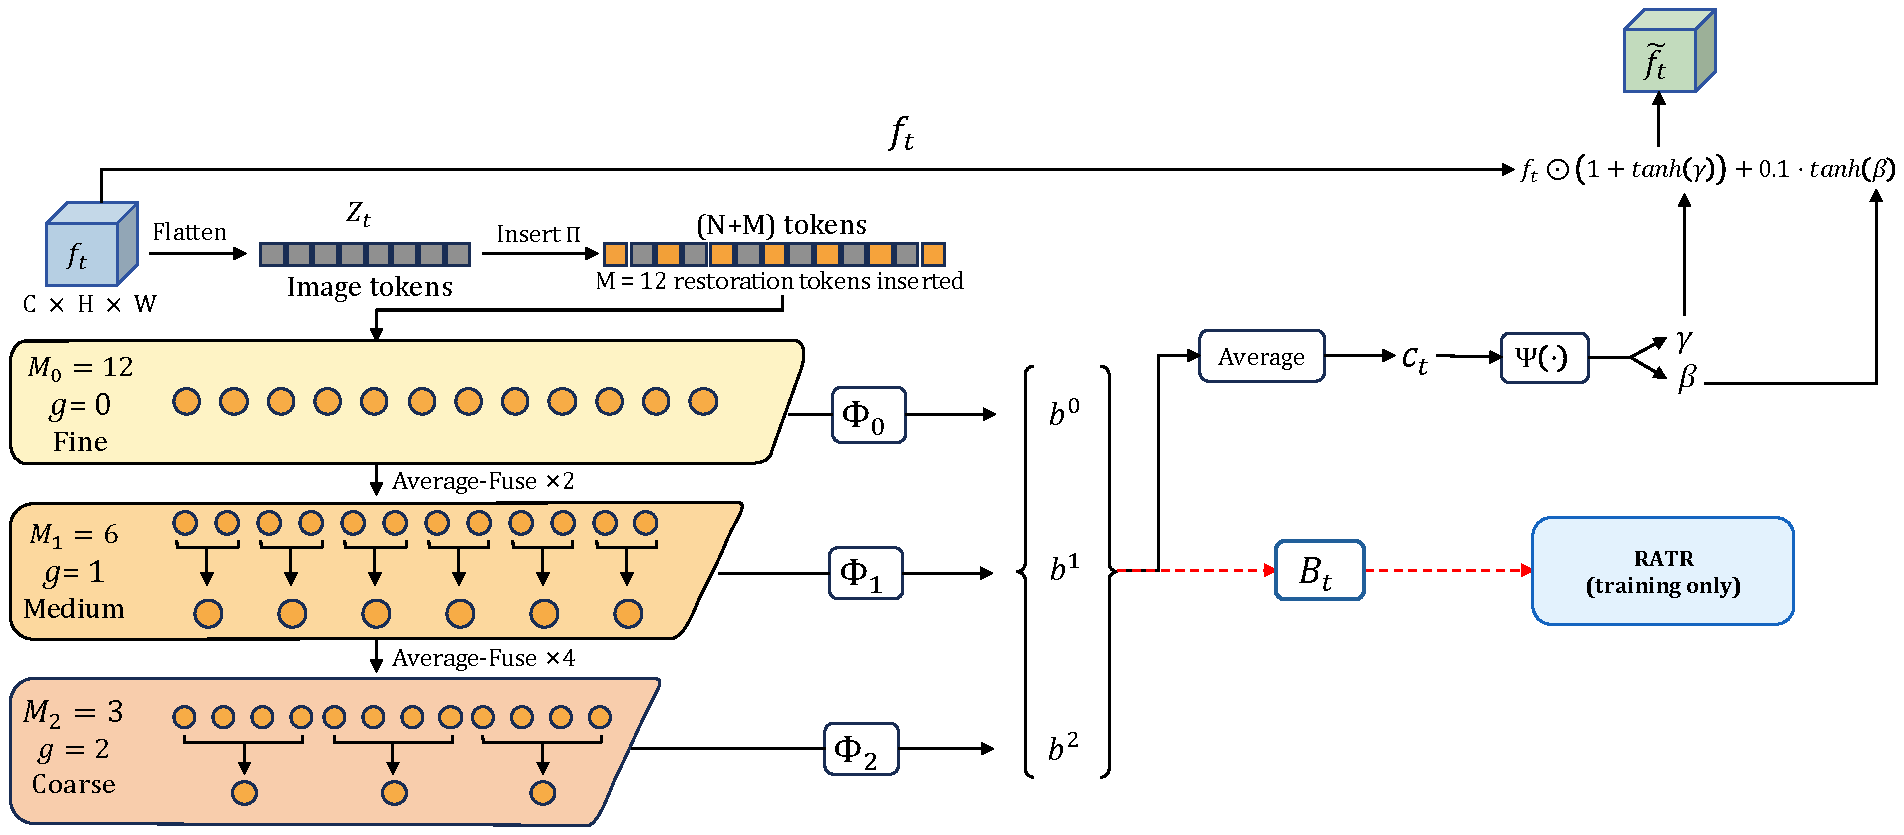
\includegraphics[width=\textwidth]{figures/Fig2_mgfe_module_detail.pdf}
\caption{Detailed Multi-Granularity Feature Extractor (MGFE) module. Propagated features are decomposed into $G=3$ restoration-token branches. The yellow, amber, and peach shaded regions denote the fine-, medium-, and coarse-granularity branches, respectively, and the red dashed path denotes the training-only connection to Ranking-Aware Triplet Regularization (RATR). $M=12$ learnable restoration tokens are inserted into image tokens, fused by progressive average fusion, and~summarized into descriptors that generate scale/shift parameters for channel-wise~recalibration.\label{fig:mgfe_detail}}
\end{figure}

The insertion $\Pi$ partitions the $N$ image tokens into $M+1$ approximately equal chunks and places one restoration token after each of the first $M$ chunks, keeping the original image-token order. Each chunk receives $\lfloor N/(M+1)\rfloor$ or $\lceil N/(M+1)\rceil$ image tokens, so the total remains exactly $N$. For~example, with~$M=3$ and $N=9$ the four chunks hold $\{3,2,2,2\}$ image tokens, and the three restoration tokens land at cumulative positions $\{3,6,9\}$ in the 12-token interleaved sequence. Spacing the tokens uniformly in this way gives them balanced receptive ranges over the full spatial~support.

MGFE then builds $G$ granularity branches by progressively fusing restoration tokens, following the progressive fusion scheme introduced in ReIDMamba~\cite{gu2025reidmamba} and adapting it to spatial restoration features. To~make every branch well defined, the~number of restoration tokens must satisfy the divisibility constraint
\begin{equation}
M = k \cdot 2^{G-1},\quad k \in \mathbb{N}^{+},
\end{equation}
so that every branch size $M_g = M/2^g$ is an integer for $g\in\{0,\ldots,G-1\}$. We use $G=3$ and $M=12$ ($k=3$) throughout; see Section~\ref{subsec:sensitivity} for alternative~configurations.

For branch $g \in \{0,\ldots,G-1\}$, MGFE fuses restoration tokens with a sampling rate of $2^g$. The~fused restoration tokens are defined as
\begin{equation}
R^{(g)}[j] =
\mathcal{F}\!\left(
\left\{R[j{\cdot}2^g+k]\right\}_{k=0}^{2^g-1}
\right),\quad
j = 0,\ldots,M_g-1,
\end{equation}
where $\mathcal{F}(\cdot)$ denotes an element-wise average over all tokens in the fusion group:
\begin{equation}
\mathcal{F}\!\left(
\left\{R[j\cdot2^g+k]\right\}_{k=0}^{2^g-1}
\right)
= \frac{1}{2^g}\sum_{k=0}^{2^g-1} R[j\cdot2^g+k]\;\in\mathbb{R}^{C_f}.
\label{eq:avg_fusion}
\end{equation}

The average is taken channel-wise. We use average fusion in the main MgfrOFR configuration because it keeps all restoration tokens contributing to the branch descriptor and prevents a single high-response token from dominating the recalibration signal. The~max-fusion variant is retained as a control in Section~\ref{subsec:ablation}; its lower full-reference scores motivate average fusion as the default. A~smaller $g$ keeps more tokens and preserves fine local detail; a larger $g$ pools a wider support and emphasizes coarse~context.

The fused tokens are re-inserted into the same image-token sequence using the same uniform-spacing insertion rule:
\begin{equation}
\widehat{Z}_t^{(g)} = \Pi\!\left(Z_t,R^{(g)}\right),
\end{equation}
and the resulting sequence is processed by a lightweight branch-specific token mixer $\Phi_g(\cdot)$:
\begin{equation}
U_t^{(g)} = \Phi_g\!\left(\widehat{Z}_t^{(g)}\right)
\in \mathbb{R}^{(N+M_g)\times C_f},
\end{equation}
where $M_g = M/2^g$. Each $\Phi_g$ consists of two sequential linear-complexity token blocks, and~each block contains a context-augmented projection sublayer and a feed-forward sublayer. The~projection sublayer first applies LayerNorm (LN), computes a global context vector by mean pooling over the token dimension, and~adds it (through a learned linear projection) to the per-token linear projection, followed by a residual connection. The~feed-forward sublayer applies LN followed by a two-layer multilayer perceptron (MLP) with Gaussian error linear unit (GELU) activation and hidden dimension $2C_f$, again with a residual connection. Formally, for~input tokens $\mathbf{h}$, each block computes
\begin{equation}
\mathbf{h}' = \mathbf{h} + W_t\,\mathrm{LN}(\mathbf{h}) + W_c\,\overline{\mathrm{LN}(\mathbf{h})},\qquad
\mathbf{h}'' = \mathbf{h}' + \mathrm{MLP}(\mathrm{LN}(\mathbf{h}')),
\end{equation}
where $\overline{(\cdot)}$ denotes mean pooling over the token dimension, $W_t,W_c\in\mathbb{R}^{C_f\times C_f}$ are learned projections, and~MLP consists of $\mathrm{Linear}(C_f\!\rightarrow\!2C_f)\!\rightarrow\!\mathrm{GELU}\!\rightarrow\!\mathrm{Linear}(2C_f\!\rightarrow\!C_f)$. The~global context term $W_c\,\overline{\mathrm{LN}(\mathbf{h})}$ gives every token an inexpensive summary of the whole sequence, so tokens exchange information at linear cost. Each branch owns its pair of token blocks and can specialize to its granularity; because the blocks are small, the~extra parameter count remains~modest.

After branch processing, we summarize each branch by averaging the updated restoration-token positions:
\begin{equation}
b_t^{(g)} =
\frac{1}{M_g}
\sum_{m=1}^{M_g}
U_t^{(g)}[\pi_m^{(M_g)}]
\in \mathbb{R}^{D},
\end{equation}
where $\{\pi_m^{(M_g)}\}_{m=1}^{M_g}$ denote the uniformly spaced insertion positions for $M_g$ tokens, and~\linebreak  $D=C_f$. Stacking all branch descriptors gives
\begin{equation}
B_t =
\left[
b_t^{(0)}, b_t^{(1)}, \ldots, b_t^{(G-1)}
\right]^\top
\in \mathbb{R}^{G \times D}.
\end{equation}

Because all descriptors come from the same propagated feature but at different fusion rates, they remain semantically aligned while differing in granularity. RATR later operates on this descriptor tensor $B_t$.

MGFE further converts the branch descriptors into a channel-wise recalibration signal. We first average the branch context,
\begin{equation}
c_t = \frac{1}{G}\sum_{g=0}^{G-1}b_t^{(g)},
\qquad
[\boldsymbol{\gamma}_t,\boldsymbol{\beta}_t] = \Psi(c_t),
\label{eq:recalibration_context}
\end{equation}
where $\Psi(\cdot)$ is a projection head consisting of $\mathrm{LayerNorm}\!\rightarrow\!\mathrm{Linear}(C_f\!\rightarrow\!2C_f)\!\rightarrow\!\mathrm{GELU}\!\rightarrow\!\mathrm{Linear}(2C_f\!\rightarrow\!2C_f)$ that outputs concatenated scale and shift vectors. The~recalibrated propagated feature is then
\begin{equation}
\widetilde{f}_t =
f_t \odot
\left(1+\tanh(\boldsymbol{\gamma}_t)\right)
+ 0.1\,\tanh(\boldsymbol{\beta}_t),
\label{eq:recalibration}
\end{equation}
where the vectors from Equation~\eqref{eq:recalibration_context} are broadcast over the spatial dimensions. The~multiplicative term $(1+\tanh(\boldsymbol{\gamma}_t))$ starts near unity, and~the small additive coefficient $0.1$ caps the shift at about $10\%$ of the $\tanh$ range, following the conservative residual scaling of FiLM-style modulation~\cite{perez2018film}. The~recalibrated feature therefore stays close to the propagated feature while the branch context remains uninformative, allowing the model to reproduce baseline behavior early in training. As~the descriptors sharpen, the~coarse branches emphasize global structure and the fine branches highlight local~damage.

MGFE produces two outputs from the same propagated feature: the branch descriptors $B_t$ and the recalibration signal $(\boldsymbol{\gamma}_t, \boldsymbol{\beta}_t)$. The~descriptors feed the ranking regularizer of Section~\ref{subsec:ratr}, while the recalibration modulates the propagated feature by granularity. Keeping them separate lets us switch off recalibration without changing the descriptors, as~in the RATR-only configuration of Section~\ref{subsec:ablation}. Explicit branches, however, do not guarantee complementary features. If~every branch ranks samples in the same order, the~branches collapse into redundant descriptors, which motivates the regularizer~below.

\subsection{Ranking-Aware Triplet Regularization (RATR)}
\label{subsec:ratr}

RATR keeps the branches from collapsing by penalizing how strongly their rankings agree. Descriptor orthogonality alone is insufficient: two branches can be orthogonal yet still order the same samples identically, leaving them redundant and undermining the balance created by MGFE. The~ordering is therefore the target. For~an anchor frame compared with nearby positives and harder negatives, RATR measures whether two branches rank that candidate set alike, using Kendall's~\cite{kendall1938measure} rank correlation coefficient made differentiable by DiffKendall~\cite{zheng2023diffkendall}. Figure~\ref{fig:ratr_detail} shows the~workflow.

\begin{figure}[t]

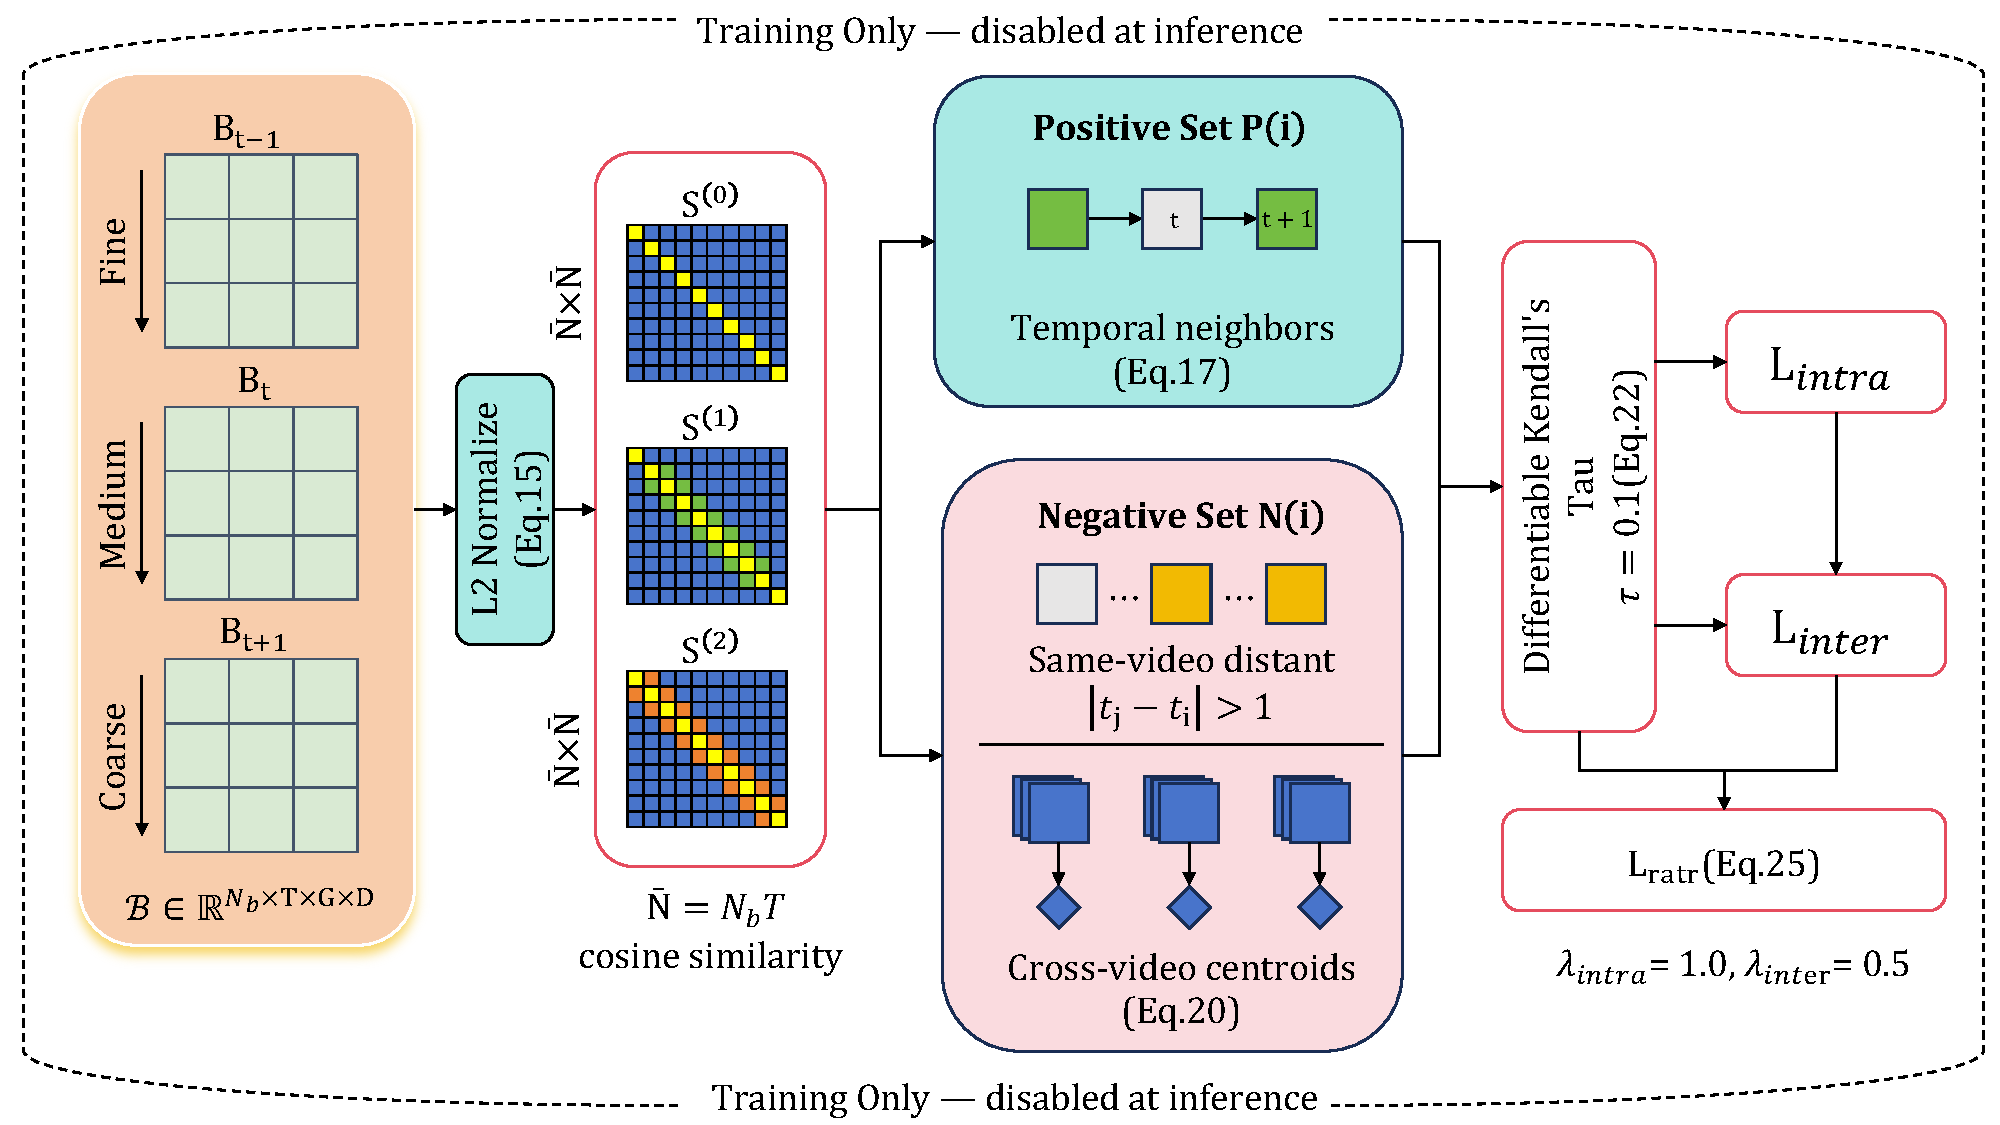
\includegraphics[width=\textwidth]{figures/Fig3_ratr_module_detail.pdf}
\caption{\hl{RATR} %MDPI: Please confirm whether the ... refers to incomplete content in this figure affects scientific understanding and if it does, please revise it.
%Author: The ellipses indicate additional negative candidates omitted from the schematic for visual clarity; they do not represent missing scientific content or processing steps. We added this explanation to the caption.
 (Ranking-Aware Triplet Regularization) compares branch-specific ranking sequences from temporal correspondences using differentiable Kendall's Tau. The cyan and pink panels denote the positive and negative candidate sets, respectively. Neighboring frames define positives, while distant same-video frames and cross-video centroids define negatives, producing $\mathcal{L}_{\text{intra}}$ and $\mathcal{L}_{\text{inter}}$ during training~only. The ellipses in the negative-set box indicate additional candidate samples omitted from the schematic for visual clarity; they do not represent missing processing steps or data.\label{fig:ratr_detail}}
\end{figure}

Let the averaged branch descriptors from Equation~\eqref{eq:mgfrofr_overview_2} be organized as a 4D tensor of shape $N_b\times T\times G\times D$, where $N_b$ is the batch size. We flatten batch and time into $\bar{N}=N_b T$ samples and normalize the descriptors branch-wise:
\begin{equation}
\widehat{b}_i^{(g)} =
\frac{b_i^{(g)}}{\|b_i^{(g)}\|_2},
\qquad
i=1,\ldots,\bar{N}.
\end{equation}

For each branch $g$, we compute a cosine-similarity matrix
\begin{equation}
\mathcal{S}^{(g)}[i,j] =
\left\langle
\widehat{b}_i^{(g)},
\widehat{b}_j^{(g)}
\right\rangle.
\end{equation}

This matrix supplies the rankings rather than serving as a supervision target itself: each anchor draws one positive ranking sequence and one negative ranking sequence from it, forming the anchor-positive-negative triplet that RATR~regularizes.

For anchor $i$, the~positive set is defined from temporal correspondences within the same clip:
\begin{equation}
\mathcal{P}(i)=
\bigl\{
j \mid v_j=v_i,\;
|t_j-t_i|=1
\bigr\},
\end{equation}
where $v_i$ and $t_i$ are the clip and frame indices of sample $i$. Adjacent frames are natural positives because the flow-guided deformable alignment in MambaOFR has already warped neighboring frames onto the anchor before MGFE runs; after alignment, they are the most reliable feature-domain proxy for true correspondences. Because~$|\mathcal{P}(i)| \le 2$ (at most one predecessor and one successor), boundary frames have only a single positive neighbor, and~we compute the intra-ranking term only on anchors that have at least two positives:
\begin{equation}
\mathcal{I}_{\text{intra}}=
\bigl\{
i \mid |\mathcal{P}(i)| \ge 2
\bigr\}.
\end{equation}

For the seven-frame clips used in training, this excludes only the first and last frame of each clip, and~every interior anchor contributes one pairwise ordering comparison to $\mathcal{L}_{\text{intra}}$. In~practice, $\mathcal{L}_{\text{intra}}$ is averaged over many valid anchors per batch, while $\mathcal{L}_{\text{inter}}$ adds a complementary signal from the richer negative~set.

Negative evidence is drawn from two harder sources: temporally distant frames inside the same clip and clip-level representatives from other clips. The~same-video negatives are
\begin{equation}
\mathcal{N}_{sv}(i)=
\bigl\{
j \mid v_j=v_i,\;
|t_j-t_i|>1
\bigr\},
\end{equation}
and the clip-level centroid for another video $v\neq v_i$ is
\begin{equation}
\bar{b}_{v}^{(g)} =
\frac{1}{|\mathcal{T}_v|}
\sum_{t\in\mathcal{T}_v}
\widehat{b}_{(v,t)}^{(g)},
\end{equation}
where $\mathcal{T}_v$ denotes the set of frame indices in clip $v$. We then construct the negative ranking sequence as
\begin{equation}
\bar{\mathcal{S}}_i^{(g)} =
\Bigl[\mathcal{S}^{(g)}[i,j]\Bigr]_{j\in\mathcal{N}_{sv}(i)}
\oplus
\Bigl[\bigl\langle \widehat{b}_i^{(g)},\,\bar{b}_v^{(g)} \bigr\rangle\Bigr]_{v\neq v_i},
\end{equation}
where $\oplus$ denotes sequence concatenation. Distant frames from the same clip are hard negatives: they share content and degradation with the anchor but are no longer immediate neighbors. Using one centroid per other clip gives a stable clip-level negative and keeps the cost linear instead of incurring the $O(\bar{N}^2)$ cost of comparing every cross-clip frame~pair.

To compare how two branches rank the same candidate set, we adopt a differentiable version of Kendall's Tau. For~sequences $p,q\in\mathbb{R}^{L}$, the~differentiable statistic is
\begin{equation}
\mathrm{DKTau}(p,q;\tau)
= \frac{1}{\binom{L}{2}}
\sum_{1\le u < v \le L}
\tanh\!\!\left(\frac{p_u-p_v}{\tau}\right)
\cdot
\tanh\!\!\left(\frac{q_u-q_v}{\tau}\right),
\label{eq:dktau}
\end{equation}
where $\tau>0$ is a temperature parameter. As~$\tau\rightarrow 0$, Equation~\eqref{eq:dktau} approaches the hard sign comparison used in the exact Kendall coefficient; as $\tau$ becomes too large, pairwise order differences are oversmoothed and gradients vanish. We set $\tau=0.1$ (see Section~\ref{subsec:sensitivity} for the sensitivity to this choice). A~lower value of $\mathrm{DKTau}(p,q;\tau)$ indicates weaker ranking correlation between branches and therefore stronger branch~complementarity.

Using Equation~\eqref{eq:dktau}, we compute the positive-ranking correlation loss as
\begin{equation}
\mathcal{L}_{\text{intra}} =
\frac{1}{|\mathcal{I}_{\text{intra}}| \binom{G}{2}}
\sum_{i\in\mathcal{I}_{\text{intra}}}
\sum_{g < g'}
\mathrm{DKTau}\!\Bigl(
\mathcal{S}^{(g)}[i,\mathcal{P}(i)],\,
\mathcal{S}^{(g')}[i,\mathcal{P}(i)];\,\tau
\Bigr),
\label{eq:loss_intra}
\end{equation}
and the negative-ranking correlation loss as
\begin{equation}
\mathcal{L}_{\text{inter}} =
\frac{1}{\bar{N} \binom{G}{2}}
\sum_{i=1}^{\bar{N}}
\sum_{g < g'}
\mathrm{DKTau}\!\Bigl(
\bar{\mathcal{S}}_i^{(g)},\,
\bar{\mathcal{S}}_i^{(g')};\,
\tau
\Bigr).
\end{equation}

The final ranking-aware regularizer is
\begin{equation}
\mathcal{L}_{\text{ratr}} =
\lambda_{\text{intra}}\,\mathcal{L}_{\text{intra}}
+ \lambda_{\text{inter}}\,\mathcal{L}_{\text{inter}}.
\label{eq:loss_ratr}
\end{equation}

Equations~\eqref{eq:loss_intra}--\eqref{eq:loss_ratr} are complementary: the intra term prevents two branches from ordering the most reliable temporal correspondences the same way, and~the inter term prevents the same collapse on harder negatives. Neither term drives the branches toward meaningless disagreement, because~the reconstruction losses still tie every branch to the same target through~MGFE.

\subsection{Symmetry Property of the~Regularizer}
\label{subsec:symmetry_property}

The representation symmetry introduced in Section~\ref{sec:introduction} has a concrete meaning in MgfrOFR. It is not a geometric symmetry of the image content but an invariance of the diversity objective under group actions that relabel branches or exchange propagation directions. Two such invariances hold, and~together they explain why the constraint is a symmetry principle rather than a balancing heuristic, as~discussed in Section~\ref{subsec:symmetry_ai}.

\begin{Property}[Branch-permutation invariance]
\hl{Both} %MDPI: we revised it to standard format, please check and confirm.
%Author: We confirm that the revision to "Both" is correct and have retained it.
 the intra term in Equation~\eqref{eq:loss_intra} and the inter term $\mathcal{L}_{\text{inter}}$ sum the differentiable Kendall statistic over unordered branch pairs $g<g'$, and~Equation~\eqref{eq:dktau} is symmetric in its arguments, $\mathrm{DKTau}(p,q;\tau)=\mathrm{DKTau}(q,p;\tau)$. Permuting the branch index of every descriptor by the same $\pi$ therefore leaves the regularizer unchanged:
\begin{equation}
\mathcal{L}_{\text{ratr}}\!\left(\{b^{(g)}\}_{g=0}^{G-1}\right)
=
\mathcal{L}_{\text{ratr}}\!\left(\{b^{(\pi(g))}\}_{g=0}^{G-1}\right),
\qquad
\forall\,\pi\in\mathcal{S}_G,
\label{eq:branch_permutation}
\end{equation}
where $\mathcal{S}_G$ is the symmetric group on the $G$ branches. In~other words, $\mathcal{L}_{\text{ratr}}$ depends only on the unordered set of pairwise branch relations, not on any branch ordering or index. Because~$\mathcal{S}_G$ has no privileged element, the~objective does not assign a preferred role to any~branch.
\end{Property}

\begin{Property}[Direction-exchange invariance]
The two propagation streams enter the regularizer only through the average $B_t=\tfrac{1}{2}(B_t^{b}+B_t^{f})$ in Equation~\eqref{eq:mgfrofr_overview_2}, which is invariant under the $\mathbb{Z}_2$ action that swaps the backward and forward descriptors, $B_t^{b}\!\leftrightarrow\!B_t^{f}$. The~objective thus treats the two temporal directions symmetrically and inherits the bidirectional symmetry of the~backbone.
\end{Property}


\textbf{\hl{Symmetry versus balancing.}%MDPI: Please confirm if the bold formatting is necessary; if not, please remove it. Please check in whole paper.
%Author: The bold formatting is intentional and has been retained because "Symmetry versus balancing" and "Scope of the claim" are inline paragraph-level headings. We checked the manuscript and retained bold formatting only where it serves the same structural purpose.
} These two invariances separate our constraint from a tuned balancing term. Balancing targets an \hl{outcome}%MDPI: Please confirm if the italics are necessary; if not, please remove them. Please check in whole paper.
%Author: The narrative italics were unnecessary, so we removed them from both "outcome" and "consequence". We checked the manuscript and retained italics only for table subgroup headings, mathematical notation, and journal-required reference formatting.
 (branches that end up contributing comparably) and is usually enforced by an asymmetric, hand-weighted penalty on individual branch magnitudes. RATR instead is built from group-invariant quantities ($\mathcal{S}_G$ on branches and $\mathbb{Z}_2$ on directions) and applies the identical constraint to every branch by construction. Balanced, complementary branches follow as a consequence of optimizing this symmetric objective, not as a separately weighted~goal.

\textbf{\hl{Scope of the claim.}} The symmetry here is functional and representation-level: an invariance of the learning objective under permutation and exchange group actions, both standard symmetry principles in machine learning, rather than a visible geometric symmetry of the restored frames. We keep this reading deliberately narrow, and~Section~\ref{subsec:symmetry_ai} relates it to the broader use of symmetry in representation~learning.

\subsection{Training~Objective}
\label{subsec:training_objective}

The generator objective combines the standard old film restoration losses used by the MambaOFR baseline with our ranking-aware regularizer. We use an $L_1$ pixel reconstruction loss $\mathcal{L}_{\mathrm{pix}}$, whose robustness for image restoration is analyzed in~\cite{zhao2017loss_restoration}, a~Visual Geometry Group (VGG)-based perceptual loss $\mathcal{L}_{\mathrm{perc}}$~\cite{johnson2016perceptual}, an~adversarial loss $\mathcal{L}_{\mathrm{gan}}$~\cite{goodfellow2014gan}, and~the ranking regularizer $\mathcal{L}_{\mathrm{ratr}}$:
\begin{equation}
\mathcal{L}_{\mathrm{total}} =
\mathcal{L}_{\mathrm{pix}}
+ \lambda_{\mathrm{perc}}\mathcal{L}_{\mathrm{perc}}
+ \lambda_{\mathrm{gan}}\mathcal{L}_{\mathrm{gan}}
+ \lambda_{\mathrm{ratr}}\mathcal{L}_{\mathrm{ratr}}.
\label{eq:loss_total}
\end{equation}

Because MGFE only augments the propagated feature stream and RATR is a pure auxiliary term, Equation~\eqref{eq:loss_total} fits into the baseline training loop without any other change. We set $\lambda_{\mathrm{perc}}=1.0$ and $\lambda_{\mathrm{gan}}=0.01$, following RTN~\cite{wan2022rtn} and MambaOFR~\cite{mao2025mambaofr}, and~use \mbox{$\lambda_{\mathrm{ratr}}=0.1$}, $\lambda_{\mathrm{intra}}=1.0$, and~$\lambda_{\mathrm{inter}}=0.5$ for the ranking term (see Section~\ref{subsec:sensitivity}). The~smaller weight on $\mathcal{L}_{\text{inter}}$ reflects the coarser ordering signal from clip-centroid negatives. Unless~stated otherwise, the~full model uses feature dimension $C_f=16$, $G=3$ branches, $M=12$ restoration tokens, channel-wise average fusion in Equation~\eqref{eq:avg_fusion}, and~differentiable Kendall temperature $\tau=0.1$.

%\input{sections/results}
\section{Experiments}
\label{sec:experiment}

We evaluate MgfrOFR under two complementary settings. Synthetic clips include ground truth and therefore support full-reference fidelity and perceptual metrics. Real archival footage lacks ground truth, so only no-reference naturalness metrics apply. We keep these settings separate throughout this section because a single merged score would mask the fidelity--naturalness trade-off that defines old film~restoration.

\subsection{Datasets and Evaluation~Metrics}
\label{subsec:datasets_metrics}

\subsubsection{Datasets}
\label{subsec:datasets}

We evaluate MgfrOFR on the SRWOV benchmark introduced with MambaOFR~\cite{mao2025mambaofr}, a~dedicated old film restoration benchmark that provides both synthetic and real-world test~sets.

For training, we use the REalistic and Dynamic Scenes (REDS) training split~\cite{nah2019reds}, which contains 240 video sequences, each with 100 frames at $720 \times 1280$ resolution. Clean REDS frames are degraded on the fly with the synthetic degradation pipeline from MambaOFR, which simulates scratches, dust, blotches, flicker, and~grain and produces paired degraded and clean training~samples.

The synthetic test set contains 30 clips rendered with the same degradation pipeline on held-out REDS sequences. Each clip has 100 frames at $720 \times 1280$ with paired ground truth, enabling full-reference scoring. The~real-world set contains 216 clips of archival footage from the 1920s to the 1960s, with~authentic mixed degradations and no ground truth. We follow the original 216-clip SRWOV protocol~\cite{mao2025mambaofr}. It spans indoor portraits, newsreel footage, conversations, and~multi-person scenes and~totals 29{,}256 frames for a broad naturalness~assessment.

\subsubsection{Evaluation~Metrics}
\label{subsec:eval_metrics}

Seven metrics cover three complementary dimensions. On~synthetic data with ground truth, we report peak signal-to-noise ratio (PSNR) and structural similarity index (SSIM)~\cite{wang2004ssim} for pixel fidelity (higher is better), learned perceptual image patch similarity (LPIPS)~\cite{zhang2018lpips} for learned perceptual distance (lower is better), and~deep image structure and texture similarity (DISTS)~\cite{ding2020dists} for joint structure-texture similarity (lower is better). On~real data without ground truth, we use natural image quality evaluator (NIQE)~\cite{mittal2012niqe} and blind/referenceless image spatial quality evaluator (BRISQUE)~\cite{mittal2012brisque} for statistical naturalness (lower is better), together with CLIP-based image quality assessment (CLIP-IQA+)~\cite{wang2023clipiqa}, which evaluates contrastive language--image pre-training (CLIP)~\cite{radford2021clip} features through learnable quality-aware prompts (higher is better). These groups probe pixel fidelity, perceptual quality, and~naturalness in~turn.

\subsection{Implementation~Details}
\label{subsec:implementation}
\unskip

\subsubsection{Training~Details}
\label{subsubsec:training_details}

We train MgfrOFR on the REDS training split~\cite{nah2019reds} with the synthetic degradation pipeline from Section~\ref{subsec:datasets}. The~optimizer is Adam~\cite{kingma2015adam} with $\beta_1=0.9$ and $\beta_2=0.99$, an~initial learning rate of $2\times10^{-4}$, and~a MultiStep schedule with milestones at 50 K, \mbox{100 K}, and~150 K iterations ($\gamma=0.5$). Training runs for $200$ K iterations on $4$ NVIDIA A100 graphics processing units (GPUs; NVIDIA Corporation, Santa Clara, CA, USA), each with 80\,GB of memory, one clip per GPU per mini-batch. Each sample is $T=7$ consecutive frames cropped to $256\times256$. We use PyTorch 2.7 with Compute Unified Device Architecture (CUDA) 12.4 and fix the random seed to 42. At~inference, RATR is off and frames are processed at full $720 \times 1280$ resolution without~cropping.

\subsubsection{Baseline Adaptation~Protocol}
\label{subsubsec:baseline_adaptation}

The comparison reuses released implementations and published settings in one unified environment. For~clarity, we make each baseline's adaptation explicit along four~axes.

\textbf{Retraining and computational budget.} Dedicated old film restoration methods (RTN, RRTN, MambaOFR) are retrained under the same REDS-based synthetic film degradation pipeline as MgfrOFR. In~particular, MambaOFR---our primary baseline---and MgfrOFR are trained with an identical 200 K-iteration schedule on the same A100-class hardware, so their computational budget for old film restoration adaptation is matched; RTN and RRTN are reproduced under the same degradation pipeline with a comparable training~budget.

\textbf{Hyper-parameter tuning.} We retain each baseline's published architecture-specific hyper-parameters rather than performing exhaustive per-baseline re-tuning. Re-tuning every method to convergence on old film restoration would be computationally prohibitive and could bias the comparison toward whichever baseline received the most tuning~effort.

\textbf{Degradation adaptation.} Generic video restoration methods (VRT, RVRT, ShiftNet) keep their published architecture and default optimization recipe; we replace only the task-specific degradation generation so that they can be trained on old film restoration inputs, and~we report them as faithfully reproduced references whose training budget follows each released~recipe.

\textbf{Reference systems.} Enhancement-oriented methods (DeOldify, OldPhoto, DeepRemaster) are not designed for paired old film restoration and are not retrained on the old film restoration pipeline; we include them strictly as reference systems to contextualize perceptual trade-offs, not as task-matched old film restoration~baselines.

The comparison is therefore a unified reproduction study under a shared degradation protocol, with~a budget-matched tier for dedicated old film restoration methods. It does not claim that every baseline has been exhaustively re-optimized for old film~restoration.

\subsection{Comparison with~State-of-the-Art}
\label{subsec:comparison_sota}

\textls[-15]{We compare MgfrOFR against nine baselines spanning dedicated old film restoration methods, general video restoration models, and~image/video enhancement approaches. The~dedicated old film restoration baselines are RTN~\cite{wan2022rtn}, RRTN~\cite{lin2024rrtn}, and~MambaOFR~\cite{mao2025mambaofr}; the general video restoration baselines are VRT~\cite{liang2024vrt}, RVRT~\cite{liang2022rvrt}, and~ShiftNet~\cite{li2023shiftnet}; and the enhancement-oriented references are DeOldify~\cite{jantic2019deoldify}, OldPhoto~\cite{wan2023oldphotopami}, and~DeepRemaster~\cite{iizuka2019deepremaster}. No-reference metrics are computed using the pyiqa library (\url{https://github.com/chaofengc/IQA-PyTorch}, accessed on 10 July 2026) under the same software~environment.}

\subsubsection{Quantitative Comparison on Synthetic~Data}

On the SRWOV synthetic benchmark with full-reference metrics (Table~\ref{tab:sota}), MgfrOFR ranks first on all four reported metrics. It reaches 27.86~dB PSNR and improves on the same-protocol MambaOFR baseline by +1.02~dB with the final average-fusion configuration. The~ranking is consistent with the architectural gap between method families: generic video restoration models include no defect handling specific to old film restoration, while frame-wise enhancement methods can break temporal~consistency.

\begin{table}[H]
\caption{\hl{Quantitative} %MDPI: please check if up/down arrow should be explained in the table footer, the below tables same as.
%Author: We added an explanation to all five affected table captions: "An upward arrow indicates that a higher value is better, whereas a downward arrow indicates that a lower value is better."
 comparison of Synthetic/Real-World Old Video (SRWOV) synthetic full-reference results under the unified reproduction protocol. The~reported metrics are peak signal-to-noise ratio (PSNR), structural similarity index (SSIM), learned perceptual image patch similarity (LPIPS), and~deep image structure and texture similarity (DISTS). Within this first comparison table, RTN denotes recurrent transformer network, RRTN denotes Recursive Recurrent Transformer Network, VRT denotes Video Restoration Transformer, and~RVRT denotes Recurrent Video Restoration Transformer. Best results are shown in \bestres{red} and second-best results in \secondres{blue}. An upward arrow indicates that a higher value is better, whereas a downward arrow indicates that a lower value is better.\label{tab:sota}}
\begin{tabularx}{\textwidth}{cCCCC}
\toprule
\textbf{Method} & \textbf{PSNR \boldmath{$\uparrow$}} & \textbf{SSIM \boldmath{$\uparrow$}} & \textbf{LPIPS \boldmath{$\downarrow$}} & \textbf{DISTS \boldmath{$\downarrow$}} \\
\midrule
ShiftNet~\cite{li2023shiftnet}          & 21.48 & 0.8234 & 0.2030 & 0.1303 \\
VRT~\cite{liang2024vrt}                 & 22.39 & 0.8631 & 0.1750 & 0.1087 \\
RVRT~\cite{liang2022rvrt}              & 22.43 & 0.8710 & 0.1655 & 0.1078 \\
DeOldify~\cite{jantic2019deoldify}      & 23.22 & 0.8923 & 0.2775 & 0.1260 \\
RRTN~\cite{lin2024rrtn}                & 24.15 & 0.9006 & 0.1082 & \secondres{0.0668} \\
OldPhoto~\cite{wan2023oldphotopami}     & 24.62 & 0.8524 & 0.2252 & 0.1144 \\
DeepRemaster~\cite{iizuka2019deepremaster} & 25.06 & \secondres{0.9185} & 0.1108 & 0.0895 \\
RTN~\cite{wan2022rtn}                   & 25.85 & 0.8869 & 0.1214 & 0.0862 \\
MambaOFR~\cite{mao2025mambaofr}        & \secondres{26.84} & 0.9153 & \secondres{0.0719} & 0.0733 \\
\midrule
MgfrOFR (Ours)                          & \bestres{27.86} & \bestres{0.9255} & \bestres{0.0600} & \bestres{0.0656} \\
\bottomrule
\end{tabularx}
\end{table}

A single average score can hide clip-level variance, so we include the paired, two-sided Wilcoxon signed-rank test over the 30 per-clip means as supporting evidence. For~the final average-fusion configuration, MgfrOFR obtains significant paired improvements over MambaOFR on all four full-reference metrics (PSNR $p=3.73\times10^{-9}$; SSIM $p=1.73\times10^{-6}$; LPIPS $p=1.86\times10^{-9}$; DISTS $p=1.92\times10^{-6}$). Per-clip evidence further shows that PSNR and DISTS improve on 29 of 30 clips, while SSIM and LPIPS improve on all 30~clips.

\subsubsection{Quantitative Comparison on Real-World~Data}

Table~\ref{tab:realworld} reports no-reference quality on the 216 real-world clips. No real-world clip has a reference, and~all methods are evaluated in the same pyiqa-based metric environment on the full 216-clip set. NIQE and BRISQUE measure statistical naturalness, while CLIP-IQA+ reflects CLIP-aligned perceptual quality; because they capture different attributes, we report each one individually instead of merging them into a single~score.

\begin{table}[H]
\caption{Real-world evaluation of no-reference quality metrics on SRWOV real footage under the same pyiqa-based metric environment. The~reported metrics are natural image quality evaluator (NIQE), blind/referenceless image spatial quality evaluator (BRISQUE), and~CLIP-based image quality assessment (CLIP-IQA+). Best results are shown in \bestres{red} and second-best results in \secondres{blue}. An upward arrow indicates that a higher value is better, whereas a downward arrow indicates that a lower value is better.\label{tab:realworld}}
\begin{tabularx}{\textwidth}{cCCC}
\toprule
\textbf{Method} & \textbf{NIQE \boldmath{$\downarrow$}} & \textbf{BRISQUE \boldmath{$\downarrow$}} & \textbf{CLIP-IQA+ \boldmath{$\uparrow$}} \\
\midrule
ShiftNet~\cite{li2023shiftnet}             & 5.71  & 42.82 & 0.3975 \\
VRT~\cite{liang2024vrt}                    & 5.66  & 42.73 & 0.3985 \\
RVRT~\cite{liang2022rvrt}                 & 5.72  & 42.64 & 0.4013 \\
DeOldify~\cite{jantic2019deoldify}         & 5.72  & 41.61 & 0.3768 \\
RRTN~\cite{lin2024rrtn}                   & 5.67  & 32.86 & 0.3969 \\
OldPhoto~\cite{wan2023oldphotopami}        & 6.56  & 30.45 & \bestres{0.4503} \\
DeepRemaster~\cite{iizuka2019deepremaster} & 5.99  & 40.62 & 0.3991 \\
RTN~\cite{wan2022rtn}                      & \secondres{5.17}  & \bestres{19.00} & 0.4163 \\
MambaOFR~\cite{mao2025mambaofr}           & 5.34  & 29.79 & \secondres{0.4351} \\
\midrule
MgfrOFR (Ours)                             & \bestres{5.12}  & \secondres{24.79} & 0.4092 \\
\bottomrule
\end{tabularx}
\end{table}

MgfrOFR obtains the best NIQE (5.12) and the second-best BRISQUE (24.79) among all compared methods, improving over MambaOFR on both NIQE (5.12 vs.\ 5.34) and BRISQUE (24.79 vs.\ 29.79). Its CLIP-IQA+ (0.4092) remains below OldPhoto (0.4503), MambaOFR (0.4351), and~RTN (0.4163). This gap is consistent with CLIP-IQA+'s tendency to favor sharper, enhancement-oriented outputs, whereas our granularity recalibration remains conservative and favors statistical naturalness. We analyze this naturalness-versus-enhancement trade-off in Section~\ref{subsec:failure}.

\subsubsection{Qualitative~Comparison}

Figure~\ref{fig:qualitative_synthetic} compares four representative synthetic scenes derived from the REalistic and Dynamic Scenes (REDS) dataset using full-frame degraded inputs and enlarged region-of-interest (ROI) crops. The~colored boxes in the input row mark local regions, and~subsequent rows compare the corresponding crops across restoration methods and the ground truth. The~method families fail in different ways. General video restoration removes part of the photometric degradation but leaves structured defects largely intact. Enhancement baselines raise contrast, yet blur or hallucinate local texture. RTN and MambaOFR clear many visible defects but still lose fine structure inside damaged regions. MgfrOFR stays closest to the ground-truth edges and textures around scratches, blotches, and~high-contrast damage while suppressing residual old-film artifacts. This behavior is consistent with the PSNR advantage in Table~\ref{tab:sota}. Supplementary Video~S1 provides side-by-side temporal comparisons in two parts: a synthetic part against the ground truth on REDS-based clips with per-frame PSNR, followed by a real-world part on SRWOV archival clips annotated with the overall no-reference NIQE and~BRISQUE.

\begin{figure}[t]
\begin{adjustwidth}{-\extralength}{0cm}
\centering
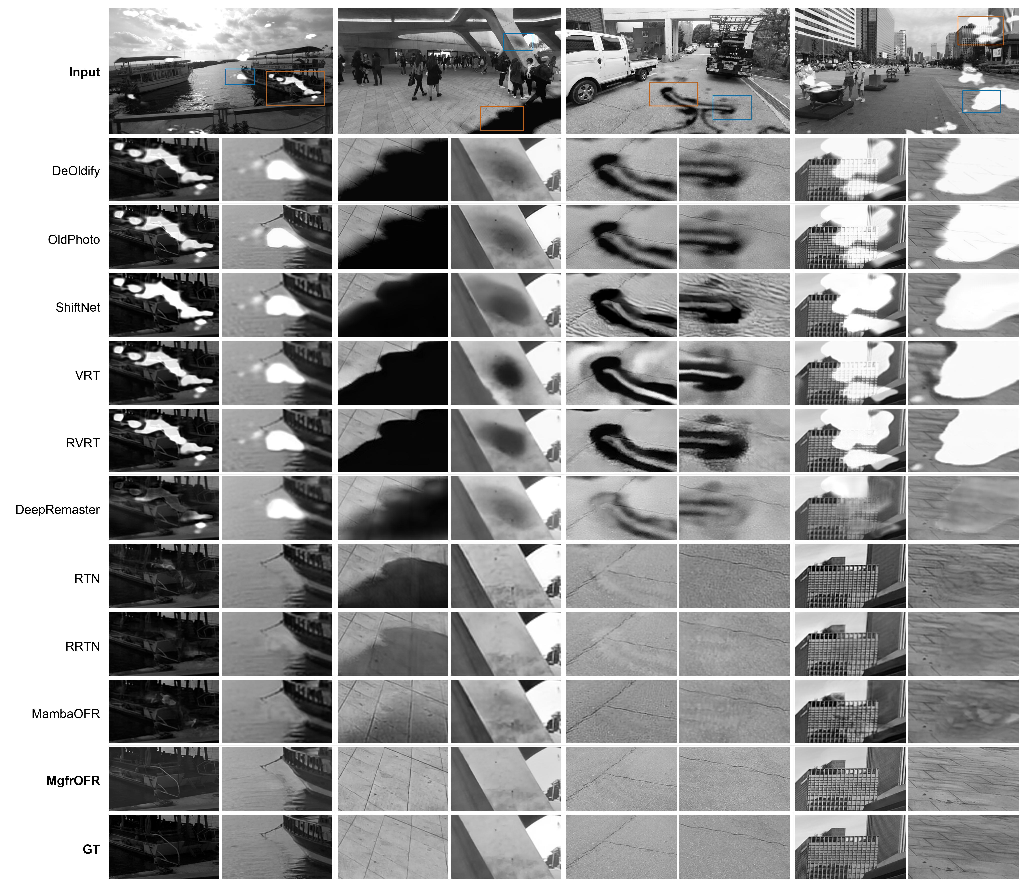
\includegraphics[width=1.21\textwidth]{figures/Fig4_SOTA_Synthetic_REDS_synthetic_Qualitative.pdf}
\end{adjustwidth}
\caption{\textls[+5]{\hl{Qualitative} %MDPI: Please confirm whether the unclear content in this figure affects scientific understanding and if it does, Please replace the image with one of a sufficiently high resolution (min. 1000 pixels width/height, or a resolution of 300 dpi or higher).
%Author: We checked Figure 4. Its source is 4110 x 3548 pixels at 600 dpi, which exceeds the requested minimum, and all scientific content is legible. No replacement is required. We also clarified the colored ROI boxes in the caption.
 comparison on four representative synthetic scenes derived from the REalistic and Dynamic Scenes (REDS) dataset. The~top row shows full degraded input frames with colored region-of-interest (ROI) boxes, and~the following rows compare enlarged ROI crops. Orange and blue boxes mark the first and second ROI crops, respectively, and~the bottom row is the ground truth (GT).}\label{fig:qualitative_synthetic}}
{\captionof*{figure}{Crops from DeOldify, OldPhoto, ShiftNet, VRT, RVRT, DeepRemaster, RTN, RRTN, MambaOFR, MgfrOFR (Ours), and~the ground truth. The~comparison shows that MgfrOFR better preserves local edges and texture details around scratches while reducing visible old-film artifacts across the selected~scenes.}}
\end{figure}
\FloatBarrier
\vspace{12pt}


Figure~\ref{fig:qualitative_realworld} compares three representative RealFilm-SRWOV real-world clips covering facial close-ups, indoor scenes, and~high-contrast local structures. Because~no ground truth is available, the~comparison focuses on visible artifact suppression, structural preservation, naturalness, and~local texture in the enlarged ROI crops. General video restoration clears part of the photometric degradation but leaves residual scratches, stains, or~contrast shifts. Enhancement baselines sharpen texture, yet can over-enhance faces, clothing, and~high-contrast boundaries. MgfrOFR maintains facial structure, fabric texture, object boundaries, and~local contrast more consistently than MambaOFR and the other old film restoration baselines, while suppressing residual old-film artifacts. These observations are consistent with the best NIQE and the BRISQUE improvement over MambaOFR in Table~\ref{tab:realworld}, while CLIP-IQA+ reflects a separate sharpness-oriented trade-off. Two failure modes remain: MgfrOFR can over-smooth very fine texture under extreme degradation. \mbox{Severe motion blur still causes flow-alignment errors.} Both are examined in Section~\ref{subsec:failure}.

\begin{figure}[t]
\begin{adjustwidth}{-\extralength}{0cm}
\centering
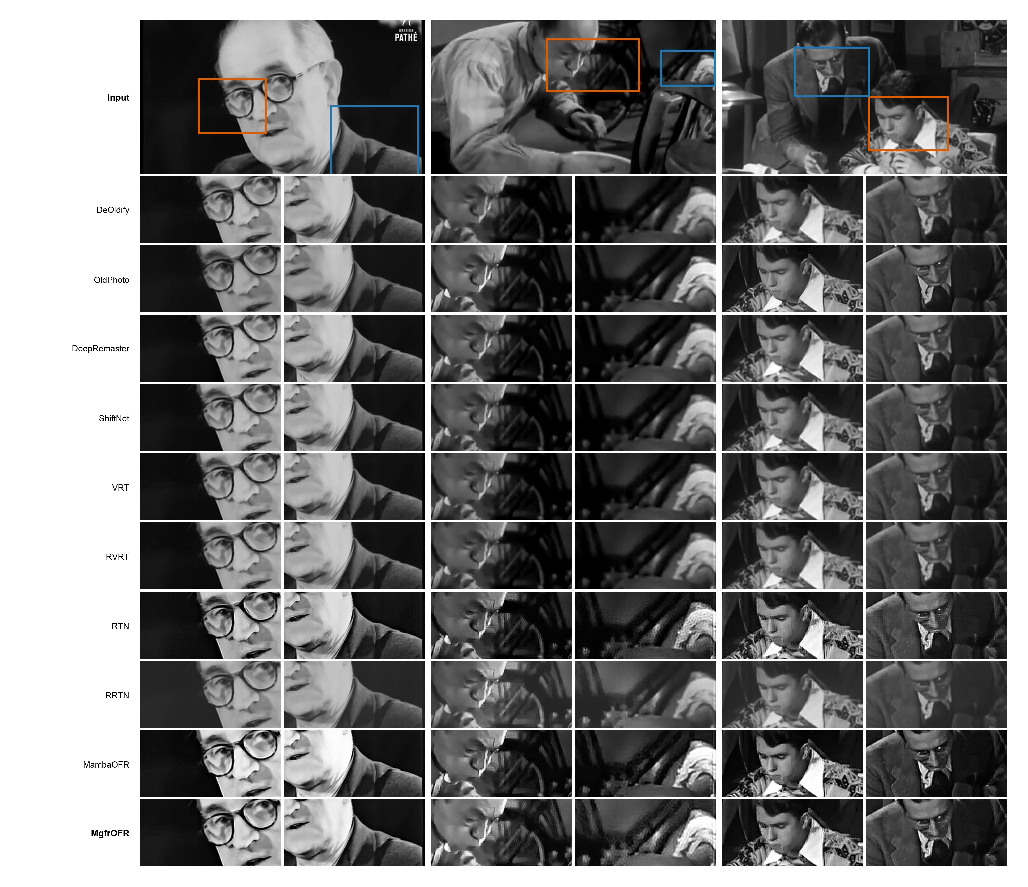
\includegraphics[width=1.18\textwidth]{figures/Fig5_SOTA_RealWorld_RealFilm_SRWOV_Qualitative.pdf}
\end{adjustwidth}
\caption{\hl{Qualitative} %MDPI: Please confirm whether the unclear content in this figure affects scientific understanding and if it does, Please replace the image with one of a sufficiently high resolution (min. 1000 pixels width/height, or a resolution of 300 dpi or higher).
%Author: We checked Figure 5. Its source is 4110 x 3548 pixels at 600 dpi, which exceeds the requested minimum, and all scientific content is legible. No replacement is required. We also clarified the colored ROI boxes in the caption.
 \hl{comparison} %MDPI: Please remove the non-English term from the figure or add a definition for it.
%Author: The text "PATHÉ" is an archival source watermark retained from the original film frame, not an untranslated manuscript term. We added this explanation to the caption and retained the watermark to preserve source integrity.
 on three representative RealFilm-SRWOV real-world clips. The~input row shows degraded frames with colored region-of-interest (ROI) boxes, and~the following rows compare enlarged ROI crops. Orange and blue boxes mark the first and second ROI crops, respectively. The text "PATHÉ" visible in the first input frame is an archival source watermark retained from the original footage, not a restoration artifact.\label{fig:qualitative_realworld}}
{\captionof*{figure}{ROI crops from DeOldify, OldPhoto, DeepRemaster, ShiftNet, VRT, RVRT, RTN, RRTN, MambaOFR, and~MgfrOFR (Ours). Because~these clips have no ground truth, the~crops compare visible local restoration details across methods. The~comparison shows that MgfrOFR suppresses residual old-film artifacts while preserving natural structure and local texture without relying on \linebreak  ground-truth~references.}}
\end{figure}
\vspace{12pt}


\subsection{Ablation~Study}
\label{subsec:ablation}

Table~\ref{tab:ablation} isolates the two contributions, MGFE recalibration and RATR regularization. These ablation values are used only for module analysis and do not replace the main comparison in Table~\ref{tab:sota}. Setting names match Figure~\ref{fig:ablation_visual}. The~+RATR-only row is a partial control: MGFE branch descriptors still serve as RATR ranking targets, but~channel-wise recalibration is switched~off.

\begin{table}[H]

\caption{Ablation study on the SRWOV synthetic benchmark. The~setting names follow Figure~\ref{fig:ablation_visual}, with~max fusion retained as a tabular control; ``MGFE'' denotes channel-wise recalibration in this table. Best results are shown in \bestres{red} and second-best results in \secondres{blue}. An upward arrow indicates that a higher value is better, whereas a downward arrow indicates that a lower value is better.\label{tab:ablation}}



\begin{adjustwidth}{-\extralength}{0cm}
\centering %% If there is a figure in wide page, please release command \centering, for Table, ``\textwidth" should be ``\fulllength"


\begin{tabularx}{\fulllength}{cCCCCCC}
\toprule
\textbf{Setting} & \textbf{MGFE} & \textbf{RATR} & \textbf{PSNR \boldmath{$\uparrow$}} & \textbf{SSIM \boldmath{$\uparrow$}} & \textbf{LPIPS \boldmath{$\downarrow$}} & \textbf{DISTS \boldmath{$\downarrow$}} \\
\midrule
MambaOFR baseline               & Off & Off & 26.84 & 0.9153 & 0.0719 & 0.0733 \\
+MGFE only                      & On  & Off & \secondres{27.75} & 0.9219 & 0.0651 & 0.0702 \\
+RATR only                      & Off & On  & 27.72 & \secondres{0.9246} & \secondres{0.0646} & \secondres{0.0696} \\
MgfrOFR (max-fusion control)   & On  & On  & 27.17 & 0.9168 & 0.0740 & 0.0773 \\
MgfrOFR (average fusion)       & On  & On  & \bestres{27.86} & \bestres{0.9255} & \bestres{0.0600} & \bestres{0.0656} \\
\bottomrule
\end{tabularx}
\end{adjustwidth}

\end{table}
\unskip
\begin{figure}[t]

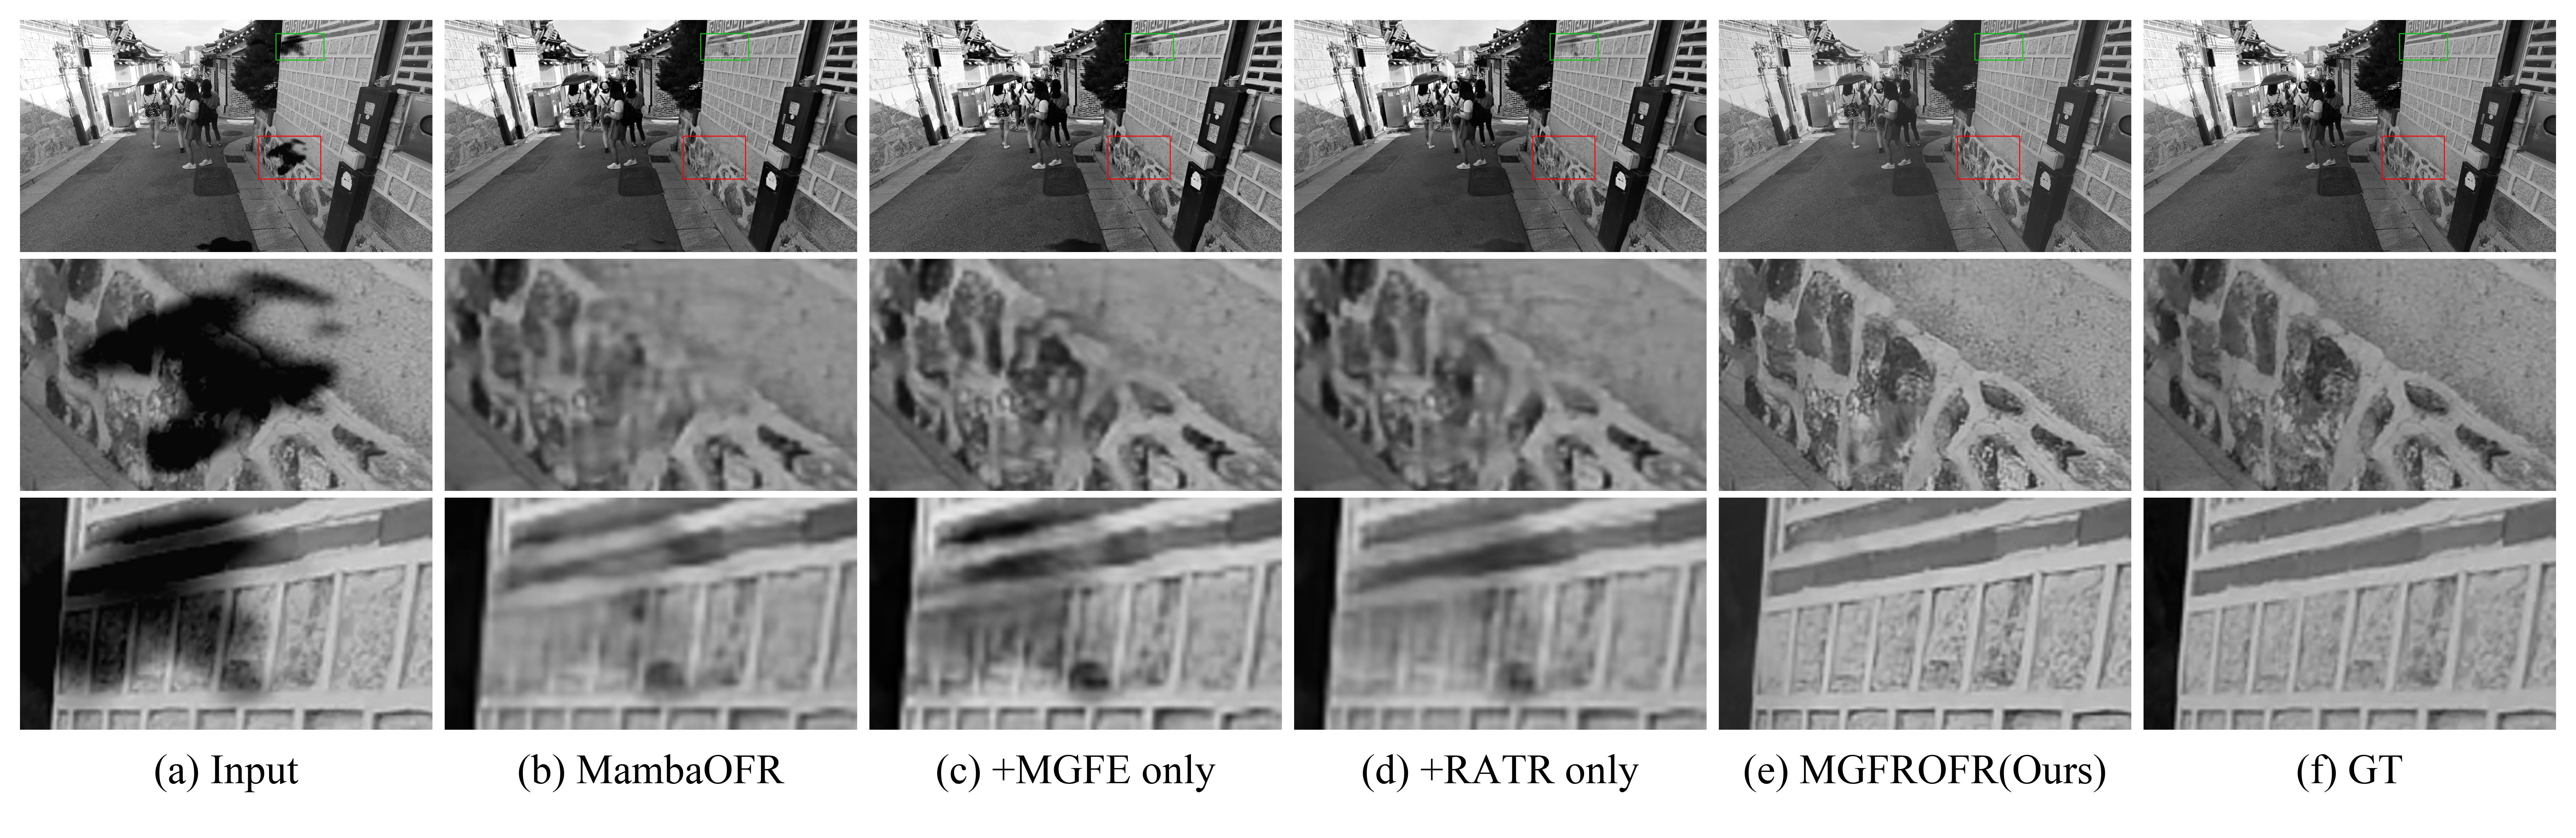
\includegraphics[width=0.99\textwidth]{figures/Fig6_Ablation_REDS_synthetic_Qualitative.jpg}
\caption{Visual ablation on REDS-based SRWOV synthetic data. (\textbf{Top row}): full frames with red and green crop boxes marking the zoom regions. (\textbf{Middle and bottom rows}): zoomed patches from the marked regions. The~restoration columns compare the MambaOFR baseline, +MGFE only, +RATR only, and~MgfrOFR with average fusion, with~the degraded input and ground truth included as references. The~max-fusion control is omitted for visual clarity. The~comparison shows that combining MGFE with RATR under average fusion yields the cleanest local restoration among the ablated configurations in Table~\ref{tab:ablation}.\label{fig:ablation_visual}}
\end{figure}


\textbf{Discussion.} Within this ablation protocol, the~full model achieves the best values for all four metrics and improves the MambaOFR baseline by +1.02~dB PSNR. Each component helps on its own, but~neither is sufficient. MGFE-only recalibration lifts the baseline yet trails the full model on LPIPS and DISTS, so recalibration alone does not deliver the best fidelity--perception balance. RATR-only regularization gives a similar PSNR gain with a better perceptual balance than MGFE-only recalibration, showing that ranking diversity is beneficial even before channel-wise feedback is enabled. Average fusion combines the two into the strongest result. The~max-fusion control shows negative synergy on all four full-reference metrics and justifies average fusion as the~default.



\subsection{Hyper-parameter~Sensitivity}
\label{subsec:sensitivity}

We report sensitivity and design-control entries only for configurations with complete evaluation records under the stated protocol. The~main MgfrOFR configuration uses average restoration-token fusion, while the earlier max-fusion configuration is retained as a fusion control. Table~\ref{tab:sensitivity_granularity} covers granularity controls, a~lower-temperature ranking control, token-insertion control, and~branch-aggregation control. The~token-insertion and branch-aggregation settings are treated as predefined max-fusion controls rather than alternatives to the average-fusion main~configuration.

\begin{table}[H]
\caption{Sensitivity and design-control results on REDS synthetic data. The~table combines a granularity sweep and fixed-size controls under the stated evaluation protocol; $M$ denotes the number of restoration tokens and $G$ denotes the number of granularity branches. MgfrOFR denotes the average-fusion main configuration, while the control rows are retained only for diagnostic comparison. Best results are shown in \bestres{red} and second-best results in \secondres{blue}. An upward arrow indicates that a higher value is better, whereas a downward arrow indicates that a lower value is better.\label{tab:sensitivity_granularity}}

\begin{adjustwidth}{-\extralength}{0cm}
\centering %% If there is a figure in wide page, please release command \centering, for Table, ``\textwidth" should be ``\fulllength"


\begin{tabularx}{\fulllength}{lCCCCCC}
\toprule
\textbf{Configuration} & \textbf{Tokens} & \textbf{Branches} & \textbf{PSNR \boldmath{$\uparrow$}} & \textbf{SSIM \boldmath{$\uparrow$}} & \textbf{LPIPS \boldmath{$\downarrow$}} & \textbf{DISTS \boldmath{$\downarrow$}} \\
\midrule
\multicolumn{7}{@{}l}{\textit{\hl{Granularity sweep}%MDPI: Please confirm if the italics are necessary; if not, please remove them. The following highlights are the same.
%Author: The italic formatting is intentional and has been retained because it distinguishes the two predefined groups of sensitivity-control rows, "Granularity sweep" and "Fixed 12-token/3-branch controls", from the individual data rows.
}} \\
$G=1$, $M=4$                      & 4  & 1 & \bestres{27.95} & \bestres{0.9263} & 0.2153 & 0.1554 \\
$G=2$, $M=8$                      & 8  & 2 & 27.49 & 0.9211 & 0.2162 & 0.1557 \\
MgfrOFR (average fusion; $G=3$, $M=12$) & 12 & 3 & \secondres{27.86} & \secondres{0.9255} & \bestres{0.0600} & \bestres{0.0656} \\
$G=4$, $M=16$                     & 16 & 4 & 27.53 & 0.9197 & 0.2169 & 0.1565 \\
\addlinespace[1pt]
\midrule
\multicolumn{7}{@{}l}{\textit{\hl{Fixed 12-token/3-branch controls}}} \\
Lower ranking temperature ($\tau=0.05$) & 12 & 3 & 26.87 & 0.9177 & 0.0672 & 0.0717 \\
Prepend token insertion               & 12 & 3 & 27.61 & 0.9234 & \secondres{0.0627} & \secondres{0.0694} \\
Max branch aggregation                & 12 & 3 & 27.55 & 0.9223 & 0.0679 & 0.0730 \\
\bottomrule
\end{tabularx}
\end{adjustwidth}
\end{table}

The granularity controls reveal a clear fidelity--perception split. The~one-branch setting achieves the highest PSNR and SSIM but much worse LPIPS and DISTS, indicating that pixel fidelity alone does not imply perceptual balance. The~average-fusion main configuration is not the PSNR maximum; however, it is the only setting here that pairs near-best fidelity with the best LPIPS and DISTS. Thus, the~perceptual gain should be attributed to the interaction among branch decomposition, token configuration, average fusion, and~RATR, not to branch count alone. The~lower-temperature control stays competitive on LPIPS and DISTS but drops fidelity, so we keep $\tau=0.1$. The~token-insertion and branch-aggregation controls both beat the max-fusion control on REDS synthetic data, yet neither overturns the average-fusion selection under the full-reference criterion. The~max-aggregation control was also run on Densely Annotated VIdeo Segmentation (DAVIS) synthetic data (26.4473 PSNR, 0.9067 SSIM, 0.0963 LPIPS, \linebreak  0.0952 DISTS) and on RealFilm\_SRWOV (5.0988 NIQE, 26.1518 BRISQUE, 0.4268 CLIP-IQA+); these real-world values are mixed, so we report them as control-scope evidence rather than as a new main-configuration~claim.



\subsection{Complexity~Analysis}
\label{subsec:complexity}

Table~\ref{tab:complexity} reports a cross-method complexity benchmark on seven-frame $256\times256$ clips. The~DeepRemaster, RTN, RRTN, and MambaOFR rows reuse frozen measurements from an earlier unified BasicOFR benchmark, whereas the MgfrOFR row was newly measured with the final average-fusion configuration. Both sets follow the same NVIDIA L40 protocol (NVIDIA Corporation, Santa Clara, CA, USA), including the same input shape, 32-bit floating-point (FP32) precision, batch size, warm-up count, and timing count; thus, the comparison is protocol-aligned but does not represent a single contemporaneous run. Floating-point operations (FLOPs) and latency are reported per seven-frame clip. The~flow-based methods include the executable optical-flow front end; DeepRemaster uses~none.

\begin{table}[H]
\caption{Computational complexity comparison under the NVIDIA L40 32-bit floating-point (FP32) unified benchmark protocol ($1\times7\times3\times256\times256$, batch size 1, three warm-up and ten timed runs). The~DeepRemaster/RTN/RRTN/MambaOFR rows reuse frozen measurements from an earlier unified BasicOFR benchmark, whereas the MgfrOFR row was newly measured under the same input-shape, FP32, batch-size, warm-up, and timing protocol using the final average-fusion configuration. Parameter counts are reported in millions (M), floating-point operations (FLOPs) in billions (G), latency in milliseconds per seven-frame clip (ms/clip), throughput in frames per second (FPS), and~peak memory in gigabytes (GB). An upward arrow indicates that a higher value is better, whereas a downward arrow indicates that a lower value is better.\label{tab:complexity}}
\begin{tabularx}{\textwidth}{cCCCCC}
\toprule
\textbf{Method} & \textbf{\footnotesize Parameters (M)} & \textbf{FLOPs (G)} & \textbf{Latency (ms/clip) \boldmath{$\downarrow$}} & \textbf{FPS \boldmath{$\uparrow$}} & \textbf{Peak Memory (GB) \boldmath{$\downarrow$}} \\
\midrule
DeepRemaster~\cite{iizuka2019deepremaster}   & 9.8781 & 914.0  & 17.9  & 391.6 & 0.35 \\
RTN~\cite{wan2022rtn}                        & 5.7351 & 2184.7 & 169.5 & 41.3  & 0.24 \\
RRTN~\cite{lin2024rrtn}                      & 7.0503 & 2782.2 & 298.4 & 23.5  & 0.75 \\
MambaOFR~\cite{mao2025mambaofr}              & 8.2984 & 2832.8 & 404.8 & 17.3  & 0.60 \\
\midrule
MgfrOFR (Ours)                              & 8.7540 & 3107.8 & 488.5 & 14.3  & 0.61 \\
\bottomrule
\end{tabularx}
\end{table}

A separate matched baseline--full-model sanity benchmark isolates the architectural overhead of the proposed design: MgfrOFR adds only 0.012 M parameters over the matched MambaOFR baseline (8.754 M vs.\ 8.742 M) and 14.094 G FLOPs per seven-frame clip (3107.781 G vs.\ 3093.687 G). In~this paired sanity run, the matched MambaOFR baseline and the final MgfrOFR configuration were measured under the same L40 FP32 protocol. These paired values are distinct from the frozen cross-method MambaOFR row reported in Table~\ref{tab:complexity}.
%Author general note: We identified two protocol-aligned complexity snapshots in the proof and now distinguish the frozen cross-method benchmark in Table~\ref{tab:complexity} from the separate paired baseline--full-model sanity benchmark in this paragraph. No complexity value was changed.

\FloatBarrier

%\input{sections/discussion}
\subsection{Analysis and~Limitations}
\label{subsec:analysis_limitations}

\subsubsection{Comparison with the Closest Prior~Work}
\label{subsec:vs_mambaofr}

MgfrOFR is built directly on top of MambaOFR~\cite{mao2025mambaofr}, so its contribution should be distinguished from the baseline backbone. We do not claim originality for bidirectional Mamba propagation, the~degradation-aware prompt block, or~the original reconstruction head. The~contribution lies in how propagated features are reorganized and regularized before~reconstruction.

Compared with MambaOFR, MgfrOFR differs in four aspects. First, the~propagated feature is no longer treated as a single restoration carrier; MGFE exposes explicit coarse-to-fine branches. Second, these branches are summarized and fed back through channel-wise recalibration rather than being used only for auxiliary supervision. Third, branch diversity is constrained by ranking correlation on temporal correspondences, rather than by an identity-based objective inherited from recognition tasks. Fourth, RATR is used only during training, so the deployment interface remains compatible with the baseline inference~pipeline.

The key value of this design is representation-level symmetry. MgfrOFR does not make object-level geometric regularity its target; instead, it examines how an AI restoration model can maintain balanced coarse-to-fine feature spaces under asymmetric film degradation. MGFE separates evidence by restoration granularity, while RATR keeps temporal-similarity rankings from becoming redundant across branches. This provides a concrete symmetry-related mechanism without overstating the mathematical scope of the~method.

\subsubsection{MGFE--RATR Synergy for Branch~Balance}
\label{subsec:synergy}

The ablation study indicates that MGFE and RATR play different roles in the full model. MGFE creates the coarse-to-fine branch structure and provides channel-wise recalibration, while RATR acts as a diversity regularizer that makes the branches more complementary (Table~\ref{tab:ablation}). In~the RATR-only configuration, MGFE branch descriptors are still computed and used as multi-granularity ranking targets; only the channel-wise scale/shift feedback is disabled. Thus, MGFE supplies the branch structure needed for coarse-to-fine feature balance, whereas RATR suppresses redundant temporal-ranking~behavior.

The asymmetric ablation behavior in Table~\ref{tab:ablation} shows that MGFE recalibration alone improves the baseline but does not reach the fidelity--perception balance of the full model. This is consistent with the perception--distortion trade-off~\cite{blau2018perception}, which establishes that optimizing a distortion measure such as PSNR does not by itself guarantee the best perceptual behavior. The~channel-wise recalibration in Equation~\eqref{eq:recalibration} is conditioned on an averaged branch context and is driven mainly by the pixel reconstruction loss. Without~a diversity constraint, the~granularity branches can converge toward similar low-frequency corrections, so the MGFE-only variant remains less effective than the full model on LPIPS and DISTS. RATR mitigates this effect by acting on branch-ranking structure rather than on pixel error. Penalizing correlated temporal rankings across branches (Equations~\eqref{eq:loss_intra}--\eqref{eq:loss_ratr}) prevents the branches from collapsing onto a single fidelity-oriented direction and preserves complementary fine-grained evidence. The~full model, therefore, gives the strongest combined fidelity and full-reference perceptual result in this~protocol.

The real-world results are consistent with this interpretation but do not prove content fidelity without ground truth. On~the SRWOV real-world test set (Table~\ref{tab:realworld}), MgfrOFR achieves the best NIQE (5.12) and improves BRISQUE relative to MambaOFR (\mbox{24.79 vs.\ 29.79}), while RTN keeps the best BRISQUE score and MgfrOFR's CLIP-IQA+ (0.4092) is lower than OldPhoto, MambaOFR, and~RTN. This pattern suggests that the multi-granularity decomposition transfers useful restoration structure beyond the synthetic training distribution, but~the no-reference gains should be interpreted as evidence of statistical naturalness rather than definitive perceptual~superiority.

\subsubsection{Branch Balance~Analysis}
\label{subsec:branch_analysis}

To verify that the three granularity branches capture complementary restoration cues rather than correlated copies of the same evidence, we analyze the pairwise cosine similarity between branch descriptors across the SRWOV synthetic test set. This analysis probes the feature space symmetry claim: balanced branches should remain comparable but not~redundant.

The full model yields lower inter-branch similarity than the MGFE-only variant\linebreak   (Figures~\ref{fig:branch_similarity} and~\ref{fig:branch_error_map}), supporting the role of RATR as the mechanism that keeps the granularity branches functionally distinct. The~RATR-only variant remains closer to the full model than to MGFE-only, showing that ranking diversity regularization already suppresses collapse even before the recalibration feedback is~enabled.
\begin{figure}[t]

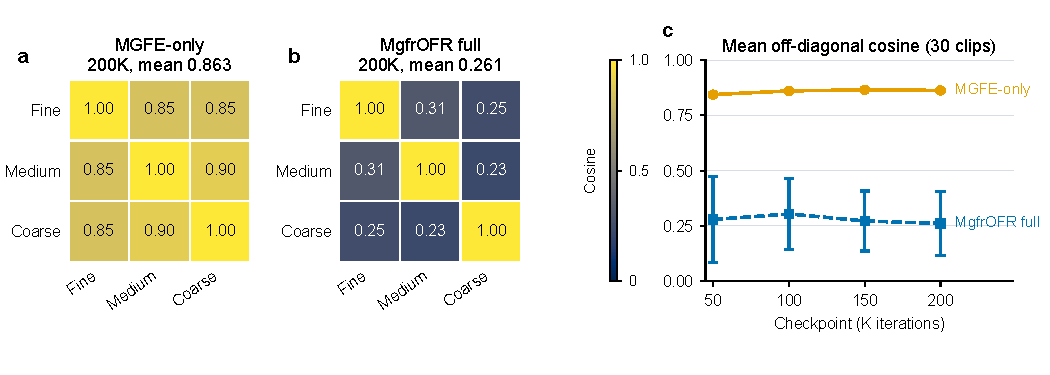
\includegraphics[width=0.98\textwidth]{figures/Fig9a_branch_similarity.pdf}
\caption{Branch balance analysis from the 30-clip REDS synthetic protocol. Panels (\textbf{a},\textbf{b}) show the final 200 K pairwise branch cosine-similarity matrices for the MGFE-only configuration and the full MgfrOFR model; panel (\textbf{c}) reports mean off-diagonal similarity with standard deviation over \mbox{30 clips} across the 50--200 K checkpoints. At~200 K, RATR reduces the mean off-diagonal similarity from $0.863\pm0.006$ to $0.261\pm0.143$, and~final pairwise off-diagonal entries drop from 0.846--0.896 to 0.226--0.310. This supports the conclusion that ranking-aware regularization prevents granularity branches from collapsing into correlated~descriptors.\label{fig:branch_similarity}}
\end{figure}
\unskip

\begin{figure}[t]

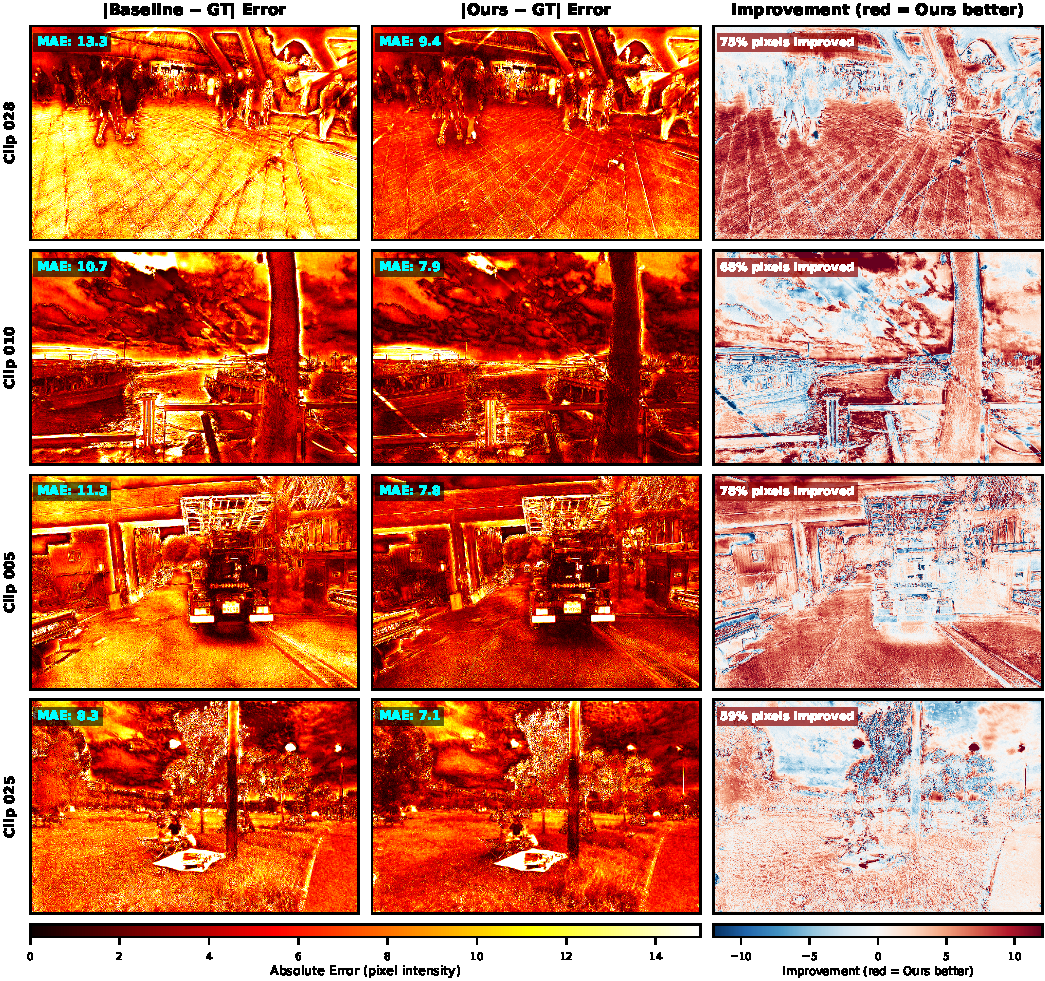
\includegraphics[width=0.98\textwidth]{figures/Fig9b_error_map.pdf}
\caption{\textls[-15]{Pixel-wise absolute-error comparison on four representative synthetic frames. Mean absolute error (MAE) is reported inside each error map. The~{(\textbf{left and middle columns})} compare $|$MambaOFR $-$ ground truth (GT)$|$ and $|$MgfrOFR $-$ GT$|$; the (\textbf{right column}) illustrates their difference, where red indicates regions in which MgfrOFR reduces the reconstruction error. The~error maps indicate that lower branch correlation translates into spatially broader restoration gains rather than isolated local~fixes.}\label{fig:branch_error_map}}
\end{figure}
\FloatBarrier

Figure~\ref{fig:branch_similarity} summarizes this contrast using the actual 30-clip branch-similarity sweep. The~heatmaps report the final 200 K pairwise branch-similarity matrices, and~the checkpoint curve reports mean off-diagonal similarity with standard deviation at 50 K, 100 K, 150 K, and~200 K iterations. In~the MGFE-only configuration, the~off-diagonal similarities remain high, indicating that the branches still encode nearly the same restoration evidence. In~the full model, these off-diagonal values stay much lower across checkpoints, showing that RATR produces a more differentiated and balanced branch~geometry.



Building on the similarity analysis, we qualitatively observe a consistent specialization pattern. The~fine-grained branch is most sensitive to localized defects such as scratches and pixel-level noise; the coarse branch emphasizes broader structural corruption such as blotches and cracks; and the medium branch occupies an intermediate role. This behavior is consistent with progressive token fusion, where fewer surviving tokens aggregate over wider spatial support. The~pixel-domain error maps in Figure~\ref{fig:branch_error_map} further indicate that this branch decorrelation translates into spatially broader restoration gains rather than isolated local~fixes.

\subsubsection{When Does MgfrOFR Struggle?}
\label{subsec:failure}

MgfrOFR's advantage is not uniform across all degradation conditions. The~ablation and sensitivity results indicate that the full model is most useful when heterogeneous degradation is present, such as structural damage co-occurring with fine scratches in the same frame. On~clips dominated by a single degradation type, such as uniform flicker without spatial damage, the~multi-granularity decomposition can add representational overhead without proportional benefit, and~the baseline or RATR-only variant may match the full model's~fidelity.

The real-world CLIP-IQA+ result highlights a trade-off between naturalness and enhancement-oriented perceptual quality. MgfrOFR's CLIP-IQA+ (0.4092) is below OldPhoto (0.4503), MambaOFR (0.4351), and~RTN (0.4163), while MgfrOFR achieves the best NIQE (5.12) and improves BRISQUE relative to MambaOFR (24.79 vs.\ 29.79). This pattern reflects the fact that different no-reference metrics measure distinct aspects of restoration quality. CLIP-IQA+ is trained on human quality annotations that correlate with sharp textures and high-contrast details~\cite{wang2023clipiqa}, favoring methods that enhance perceptual sharpness through learned global priors. NIQE and BRISQUE instead measure statistical deviation from natural image distributions and penalize artifacts introduced by texture hallucination. MgfrOFR's granularity-based recalibration operates conservatively on the propagated feature stream, which appears to preserve statistical naturalness while providing less texture enhancement than the stronger CLIP-IQA+ baselines. For~archival restoration, NIQE/BRISQUE may be more relevant proxies when content fidelity is prioritized, but~human evaluation is needed to validate that~preference.

\subsubsection{Limitations, Threats to Validity, and~Future~Work}
\label{subsec:limitations}

\paragraph{Threats to Validity}
Five threats affect the interpretation of the results. \textbf{\hl{Dataset threat}%MDPI: Please confirm if the bold formatting is necessary; if not, please remove it. The following highlights are the same.
%Author: The bold formatting is intentional and has been retained because the short labels distinguish the five threat categories within a single paragraph.
}: all training uses synthetic degradation applied to REDS clips, which introduces a synthetic-to-real domain gap and may limit generalization to archival footage with correlated degradation chains not modeled by the pipeline. \textbf{\hl{Metric threat}}: evaluation relies on PSNR/SSIM/LPIPS/DISTS for synthetic full-reference assessment and no-reference metrics for real-world assessment; these metrics emphasize different aspects of quality and may not fully align with human perceptual judgments. \textbf{Human-evaluation threat}: the study does not include an expert reader study with film-restoration practitioners or archivists, so the practical value of \mbox{improvements} on authentic footage is inferred from proxy metrics and qualitative inspection. \textbf{Baseline threat}: three baselines (VRT, RVRT, ShiftNet) required adaptation from video restoration to old-film-specific degradation, which preserves their architectures but may not reflect their optimal performance under a different training regime. \textbf{Synthetic-to-real threat}: the real-world evaluation lacks ground truth, so improvements in NIQE/BRISQUE reflect statistical naturalness rather than verified content fidelity, and~the absence of external validation on additional datasets limits the generalization~claim.

\paragraph{Limitations and Future Work}
RATR adds training-time cost because it requires branch-wise similarity matrices over the batch-time descriptor set $\bar{N}=N_bT$. Its dominant cost therefore grows approximately quadratically in $\bar{N}$. Longer clips or larger effective batch-time products would make this quadratic term more pronounced, so gradient checkpointing or selective ranking construction, such as sampling a subset of anchors per iteration, will be needed for larger training settings. The~second limitation is the synthetic-to-real domain gap caused by REDS-based training degradation. Although~the real-world NIQE/BRISQUE results are encouraging, authentic archival footage can contain correlated degradation chains that synthetic pipelines do not model. The~third limitation is evaluation scope: validation is limited to SRWOV, and~additional archival datasets plus human evaluation would strengthen claims about~generalization.

Promising extensions include adaptive branch activation conditioned on degradation severity, frequency-aware branch specialization that assigns structural recovery and texture restoration to dedicated branches, and~joint old film restoration and colorization frameworks for archival digitization and cultural heritage restoration workflows~\cite{kokaram2004missing}.

%\input{sections/conclusion}
\section{Conclusions}
\label{sec:conclusion}

We presented MgfrOFR, a~Mamba-based old film restoration framework that augments MambaOFR with explicit multi-granularity feature balancing. The~Multi-Granularity Feature Extractor (MGFE) reorganizes propagated features into coarse-to-fine restoration-token branches and recalibrates the spatial stream through channel-wise feedback, while Ranking-Aware Triplet Regularization (RATR) discourages branch collapse by penalizing correlated temporal-similarity rankings during~training.

With the final average-fusion configuration on the synthetic benchmark, MgfrOFR achieves the strongest full-reference scores among the tested baselines, improving PSNR by 1.02~dB over MambaOFR (27.86~dB vs.\ 26.84~dB). On~216 real-world archival clips, MgfrOFR obtains the lowest NIQE (5.12), improves BRISQUE over MambaOFR \mbox{(24.79 vs.\ 29.79)}, and~shows a lower CLIP-IQA+ value (0.4092) than the sharper enhancement-oriented references and old film restoration baselines. Because~the real-world setting lacks ground truth, these no-reference gains should be interpreted as evidence of improved statistical naturalness rather than definitive proof of perceptual superiority. The~ablation study further shows that MGFE and RATR are complementary: MGFE alone improves the baseline but remains weaker than the full model on full-reference perceptual metrics, whereas the full model gives the best combined result when branch diversity is explicitly enforced through RATR and average~fusion.

These results suggest that representation-level branch balance is a useful inductive bias for heterogeneous-degradation video restoration and practical archival digitization workflows. The~main implication is that feature space symmetry and temporally coordinated ranking behavior can improve restoration under degradation-induced asymmetry without changing the baseline inference interface. Several limitations remain: the method inherits the synthetic-to-real domain gap of REDS-based training; RATR adds a training-time cost whose dominant batch-time ranking term grows approximately quadratically with the descriptor set; and evaluation is limited to the SRWOV benchmark and no-reference proxies on authentic footage. Future work will focus on adaptive branch activation conditioned on degradation severity, frequency-aware branch specialization for structural recovery and texture restoration, lighter ranking constructions such as selective anchor sampling, human-in-the-loop evaluation, and~broader validation on additional archival~benchmarks.
%Author general note: We removed the previously stated exact training-time increase because it was not supported by a retained training-time log. We retained only the qualitative quadratic-cost statement supported by the branch-wise similarity construction.


\vspace{6pt}


\supplementary{The following supporting information can be downloaded at: \linksupplementary{s1},  Video S1: side-by-side old-film restoration comparison in two parts. The~first part uses REDS-synthetic clips with paired ground truth (GT) and per-frame PSNR (Input, MambaOFR, MgfrOFR, GT); the second part uses real-world SRWOV archival clips annotated with the overall no-reference NIQE/BRISQUE (Input, MambaOFR, MgfrOFR).}

\authorcontributions{Conceptualization, F.C. and Y.D.; methodology, F.C.; software, F.C.; validation, F.C. and Q.Z.; formal analysis, F.C.; investigation, F.C.; resources, K.Y., L.C. and Y.D.; data curation, F.C.; writing---original draft preparation, F.C.; writing---review and editing, Q.Z., K.Y., L.C. and Y.D.; visualization, F.C.; supervision, Y.D.; project administration, Y.D.; funding acquisition, Y.D. All authors have read and agreed to the published version of the~manuscript.}

\funding{This research received no external~funding.}

\institutionalreview{Not applicable.}

\informedconsent{Not applicable.}



\dataavailability{The training data follow the public REDS benchmark and the SRWOV protocol described by MambaOFR. The~manuscript source and figures are included in this submission package. Code, configurations, and~evaluation scripts for this study are publicly available at \url{https://github.com/wscffaa/MgfrOFR}  (\hl{accessed on 10 July 2026}%MDPI: Please add the access date (format: Date Month Year), e.g., accessed on 1 January 2020.
%Author: We added the requested access date, 10 July 2026, and verified that the repository is publicly accessible without authentication at the stated URL.
). Public benchmark data should be obtained from the original REDS and SRWOV/MambaOFR sources; no new dataset is redistributed in this work.}

\acknowledgments{The authors thank the developers of MambaOFR for releasing their code and pretrained models. During~the preparation of this manuscript, the~authors used OpenAI Codex (GPT-5; \url{https://openai.com/codex/}; \hl{accessed on 1 July 2026}%MDPI: please check if missing website link before it or remove this access date.
%Author: We added the official OpenAI Codex website link (https://openai.com/codex/) before the access date and retained "accessed on 1 July 2026".
) solely for language polishing, including grammar, spelling, punctuation, and~wording clarity. The~authors reviewed and edited the output and take full responsibility for the content of this~publication.}

\conflictsofinterest{The authors declare no conflicts of~interest.}

\clearpage
\abbreviations{Abbreviations}{
The following key abbreviations are used in this manuscript:\\

\noindent
\begin{tabularx}{\textwidth}{@{}lX}
MgfrOFR & Multi-Granularity Feature Decomposition with Ranking-Aware Regularization for Old Film~Restoration\\
MGFE & Multi-Granularity Feature~Extractor\\
RATR & Ranking-Aware Triplet~Regularization\\
RTN & Recurrent Transformer~Network\\
RRTN & Recursive Recurrent Transformer~Network\\
SSM & State Space~Model\\
DPB & Degradation-Aware Prompt~Block\\
DCN & Deformable Convolutional~Network\\
PSNR & Peak Signal-to-Noise~Ratio\\
SSIM & Structural Similarity~Index\\
LPIPS & Learned Perceptual Image Patch~Similarity\\
DISTS & Deep Image Structure and Texture~Similarity\\
NIQE & Natural Image Quality~Evaluator\\
BRISQUE & Blind/Referenceless Image Spatial Quality~Evaluator\\
CLIP & Contrastive Language--Image Pre-Training\\
CLIP-IQA+ & CLIP-based Image Quality Assessment (enhanced)\\
SRWOV & Synthetic/Real-World Old~Video\\
REDS & REalistic and Dynamic~Scenes\\
DAVIS & Densely Annotated VIdeo~Segmentation\\
AI & Artificial~Intelligence\\
RGB & Red--Green--Blue\\
ROI & Region of~Interest\\
LN & Layer~Normalization\\
MLP & Multilayer~Perceptron\\
GELU & Gaussian Error Linear~Unit\\
VGG & Visual Geometry~Group\\
CUDA & Compute Unified Device~Architecture\\
FLOPs & Floating-Point~Operations\\
FPS & Frames per~Second\\
GT & Ground~Truth\\
GPU & Graphics Processing~Unit\\
\end{tabularx}
}

\begin{adjustwidth}{-\extralength}{0cm}
\reftitle{References}
%\bibliography{references}
\begin{thebibliography}{999}

\bibitem[Iizuka and Simo-Serra(2019)]{iizuka2019deepremaster}
Iizuka, S.; Simo-Serra, E.
\newblock {DeepRemaster}: Temporal Source-Reference Attention Networks for
  Comprehensive Video Enhancement.
\newblock {\em ACM Trans. Graph.} {\bf 2019}, {\em 38},~1--13.
\newblock {\url{https://doi.org/10.1145/3355089.3356570}}.

\bibitem[Wan et~al.(2022)Wan, Zhang, Li, Liu, Chen, and Loy]{wan2022rtn}
Wan, Z.; Zhang, B.; Li, D.; Liu, Y.; Chen, J.; Loy, C.C.
\newblock Bringing Old Films Back to Life.
\newblock In \emph{Proceedings of the IEEE/CVF Conference on Computer Vision and
  Pattern Recognition (CVPR), \hl{New Orleans, LA, USA, 18--24 June} %MDPI: We added the location and date of the conference. Please confirm.
%Author: We confirm that the added conference location and dates, New Orleans, LA, USA, 18--24 June 2022, are correct.
  2022}; \hl{IEEE:} %MDPI: we added the name of the publisher, please check and confirm.
%Author: We confirm that IEEE is the correct publisher and have retained the added publisher information.
 New York, NY, USA, 2022; \linebreak  pp. 17694--17703.
\newblock {\url{https://doi.org/10.1109/CVPR52688.2022.01717}}.

\bibitem[Lin and Simo-Serra(2024)]{lin2024rrtn}
Lin, S.; Simo-Serra, E.
\newblock Restoring Degraded Old Films with Recursive Recurrent Transformer
  Networks.
\newblock In Proceedings of the Proceedings of the IEEE/CVF Winter Conference
  on Applications of Computer Vision, \hl{Waikoloa, HI, USA, 3--8 January} 2024; \linebreak  pp. 6704--6714.
\newblock {\url{https://doi.org/10.1109/WACV57701.2024.00658}}.

\bibitem[Mao et~al.(2025)Mao, Zhang, Wan, Li, and Loy]{mao2025mambaofr}
Mao, T.; Zhang, L.; Wan, Z.; Li, G.; Loy, C.C.
\newblock {MambaOFR}: Old Film Restoration with State Space Model.
\newblock In \emph{Proceedings of the IEEE/CVF Conference on Computer Vision and
  Pattern Recognition (CVPR), \hl{Nashville, TN, USA, 10--17 June} 2025}; IEEE: New York, NY, USA, 2025; pp. 4622--4630.
\newblock {\url{https://doi.org/10.1109/CVPR52734.2025.02611}}.

\bibitem[Gu and Dao(2024)]{gu2024mamba}
Gu, A.; Dao, T.
\newblock Mamba: Linear-Time Sequence Modeling with Selective State Spaces.
\newblock In Proceedings of the Conference on Language Modeling (COLM), \hl{Philadelphia, PA, USA, 7--9 October}  2024\hl{.} %MDPI: we removed unnecessary information, please confirm.
%Author: We confirm the revised reference format and the removal of the unnecessary information. The conference location and dates are correct and have been retained.
  \url{ 	
https://doi.org/10.48550/arXiv.2312.00752}.
%\newblock Published at COLM 2024; OpenReview venue page used as canonical
%  landing page.

\bibitem[Guo et~al.(2024)Guo, Li, Dai, Ouyang, Ren, and Xia]{guo2024mambair}
Guo, H.; Li, J.; Dai, T.; Ouyang, Z.; Ren, X.; Xia, S.T.
\newblock {MambaIR}: A Simple Baseline for Image Restoration with State-Space
  Model.
\newblock In \emph{Proceedings of the European Conference on Computer Vision (ECCV), \hl{Milan, Italy,  29 September--4 October}  2024}; Springer: Cham, Switzerland, 2024; pp. 222--241.
 \newblock {\url{https://doi.org/10.1007/978-3-031-72649-1_13}}.

\bibitem[Lin et~al.(2017)Lin, Doll{\'a}r, Girshick, He, Hariharan, and
  Belongie]{lin2017fpn}
Lin, T.Y.; Doll{\'a}r, P.; Girshick, R.; He, K.; Hariharan, B.; Belongie, S.
\newblock Feature Pyramid Networks for Object Detection.
\newblock In \emph{Proceedings of the IEEE/CVF Conference on Computer Vision and
  Pattern Recognition (CVPR), \hl{Honolulu, HI, USA, 21--26 July} 2017}; IEEE: New York, NY, USA,  2017; pp. 936--944.
\newblock {\url{https://doi.org/10.1109/CVPR.2017.106}}.

\bibitem[Wang et~al.(2021)Wang, Sun, Cheng, Jiang, Deng, Zhao, Liu, Mu, Tan,
  Wang, Liu, and Xiao]{wang2021hrnet}
Wang, J.; Sun, K.; Cheng, T.; Jiang, B.; Deng, C.; Zhao, Y.; Liu, D.; Mu, Y.;
  Tan, M.; Wang, X.;  et~al.
\newblock Deep High-Resolution Representation Learning for Visual Recognition.
\newblock {\em IEEE Trans. Pattern Anal. Mach. Intell.}
  {\bf 2021}, {\em 43},~3349--3364.
\newblock {\url{https://doi.org/10.1109/TPAMI.2020.2983686}}.

\bibitem[Sun et~al.(2018)Sun, Zheng, Yang, Tian, and Wang]{sun2018pcb}
Sun, Y.; Zheng, L.; Yang, Y.; Tian, Q.; Wang, S.
\newblock Beyond Part Models: Person Retrieval with Refined Part Pooling.
\newblock In \emph{Proceedings of the European Conference on Computer Vision (ECCV)};
  Springer: Cham, Switzerland,  2018; pp. 480--496.
\newblock {\url{https://doi.org/10.1007/978-3-030-01225-0_30}}.

\bibitem[Wang et~al.(2018)Wang, Yuan, Chen, Li, and Zhou]{wang2018mgn}
Wang, G.; Yuan, Y.; Chen, X.; Li, J.; Zhou, X.
\newblock Learning Discriminative Features with Multiple Granularities for
  Person Re-Identification.
\newblock In \emph{Proceedings of the ACM International Conference on Multimedia
  (MM)}; \hl{Association for Computing Machinery:} New York, NY, USA,  2018; pp. 274--282.
\newblock {\url{https://doi.org/10.1145/3240508.3240552}}.

\bibitem[Gu et~al.(2026)Gu, Yang, Pu, Han, and Ding]{gu2025reidmamba}
Gu, H.; Yang, Q.; Pu, L.; Han, S.; Ding, Y.
\newblock {ReIDMamba}: Learning Discriminative Features with Visual State Space
  Model for Person Re-Identification.
\newblock {\em IEEE Trans. Multimed.} {\bf 2026}, \emph{Early access}.
 \newblock {\url{https://doi.org/10.1109/TMM.2026.3668499}}.

\bibitem[Kokaram(2004)]{kokaram2004missing}
Kokaram, A.C.
\newblock On Missing Data Treatment for Degraded Video and Film Archives: {A}
  Survey and a New {Bayesian} Approach.
\newblock {\em IEEE Trans. Image Process.} {\bf 2004}, {\em
  13},~397--415.
\newblock {\url{https://doi.org/10.1109/TIP.2004.823815}}.

\bibitem[Dabov et~al.(2007)Dabov, Foi, Katkovnik, and
  Egiazarian]{dabov2007bm3d}
Dabov, K.; Foi, A.; Katkovnik, V.; Egiazarian, K.
\newblock Image Denoising by Sparse {3-D} Transform-Domain Collaborative
  Filtering.
\newblock {\em IEEE Trans. Image Process.} {\bf 2007}, {\em
  16},~2080--2095.
\newblock {\url{https://doi.org/10.1109/TIP.2007.901238}}.

\bibitem[He et~al.(2013)He, Sun, and Tang]{he2013guided}
He, K.; Sun, J.; Tang, X.
\newblock Guided Image Filtering.
\newblock {\em IEEE Trans. Pattern Anal. Mach. Intell.}
  {\bf 2013}, {\em 35},~1397--1409.
\newblock {\url{https://doi.org/10.1109/TPAMI.2012.213}}.

\bibitem[Wang et~al.(2019)Wang, Chan, Yu, Dong, and Loy]{wang2019edvr}
Wang, X.; Chan, K.C.; Yu, K.; Dong, C.; Loy, C.C.
\newblock {EDVR}: Video Restoration with Enhanced Deformable Convolutional
  Networks.
\newblock In Proceedings of the IEEE/CVF Conference on
  Computer Vision and Pattern Recognition Workshops, \hl{Long Beach, CA, USA, 16--17 June} 2019; pp. 1954--1963.
\newblock {\url{https://doi.org/10.1109/CVPRW.2019.00247}}.

\bibitem[Chan et~al.(2021)Chan, Wang, Yu, Dong, and Loy]{chan2021basicvsr}
Chan, K.C.; Wang, X.; Yu, K.; Dong, C.; Loy, C.C.
\newblock {BasicVSR}: The Search for Essential Components in Video
  Super-Resolution and Beyond.
\newblock In Proceedings of the IEEE/CVF Conference on
  Computer Vision and Pattern Recognition, \hl{Nashville, TN, USA, 20--25 June} 2021; pp. 4945--4954.
\newblock {\url{https://doi.org/10.1109/CVPR46437.2021.00491}}.

\bibitem[Chan et~al.(2022)Chan, Zhou, Xu, and Loy]{chan2022basicvsrpp}
Chan, K.C.; Zhou, S.; Xu, X.; Loy, C.C.
\newblock {BasicVSR++}: Improving Video Super-Resolution with Enhanced
  Propagation and Alignment.
\newblock In Proceedings of the IEEE/CVF Conference on
  Computer Vision and Pattern Recognition, \hl{New Orleans, LA, USA, 18--24 June} 2022; pp. 5962--5971.
\newblock {\url{https://doi.org/10.1109/CVPR52688.2022.00588}}.

\bibitem[Liang et~al.(2024)Liang, Cao, Fan, Zhang, Ranjan, Li, Timofte, and
  {Van Gool}]{liang2024vrt}
Liang, J.; Cao, J.; Fan, Y.; Zhang, K.; Ranjan, R.; Li, Y.; Timofte, R.; {Van
  Gool}, L.
\newblock {VRT}: A Video Restoration Transformer.
\newblock {\em IEEE Trans. Image Process.} {\bf 2024}, {\em
  33},~2171--2182.
\newblock {\url{https://doi.org/10.1109/TIP.2024.3372454}}.

\bibitem[Liang et~al.(2022)Liang, Fan, Xiang, Ranjan, Ilg, Green, Cao, Zhang,
  Timofte, and {Van Gool}]{liang2022rvrt}
Liang, J.; Fan, Y.; Xiang, X.; Ranjan, R.; Ilg, E.; Green, S.; Cao, J.; Zhang,
  K.; Timofte, R.; {Van Gool}, L.
\newblock Recurrent Video Restoration Transformer with Guided Deformable
  Attention.
\newblock In \emph{Proceedings of the Neural Information Processing Systems
  (NeurIPS)}; \hl{Neural Information Processing Systems Foundation, Inc. (NeurIPS)}: Red Hook, NY, USA,  2022; pp. 378--393.
 \newblock {\url{https://doi.org/10.52202/068431-0028}}.

\bibitem[Lin et~al.(2024)Lin, He, Chen, Lyu, Dai, Yu, Qiao, Ouyang, and
  Dong]{lin2024diffbir}
Lin, X.; He, J.; Chen, Z.; Lyu, Z.; Dai, B.; Yu, F.; Qiao, Y.; Ouyang, W.;
  Dong, C.
\newblock {DiffBIR}: Toward Blind Image Restoration with Generative Diffusion
  Prior.
\newblock In \emph{Proceedings of the European Conference on Computer Vision (ECCV)}; \hl{Springer: Cham, Switzerland,}
  2024.
\newblock {\url{https://doi.org/10.1007/978-3-031-73202-7_25}}.

\bibitem[Yu et~al.(2024)Yu, Gu, Li, Hu, Kong, Wang, He, Qiao, and
  Dong]{yu2024supir}
Yu, F.; Gu, J.; Li, Z.; Hu, J.; Kong, X.; Wang, X.; He, J.; Qiao, Y.; Dong, C.
\newblock Scaling Up to Excellence: Practicing Model Scaling for
  Photo-Realistic Image Restoration in the Wild.
\newblock In Proceedings of the IEEE/CVF Conference on
  Computer Vision and Pattern Recognition (CVPR),  \hl{Seattle, WA, USA, 16--22 June} 2024; pp. 25669--25680.

\bibitem[Wu et~al.(2024)Wu, Yang, Sun, Zhang, Li, and Zhang]{wu2024seesr}
Wu, R.; Yang, T.; Sun, L.; Zhang, Z.; Li, S.; Zhang, L.
\newblock {SeeSR}: Towards Semantics-Aware Real-World Image Super-Resolution.
\newblock In Proceedings of the IEEE/CVF Conference on
  Computer Vision and Pattern Recognition (CVPR), \hl{Seattle, WA, USA, 16--22 June} 2024; pp. 25456--25467.

\bibitem[Gu et~al.(2022)Gu, Goel, and R{\'e}]{gu2022s4}
Gu, A.; Goel, K.; R{\'e}, C.
\newblock Efficiently Modeling Long Sequences with Structured State Spaces.
\newblock In Proceedings of the International Conference on Learning
  Representations (ICLR), \hl{Virtual,  25--29 April} 2022.
  \url{ 	
https://doi.org/10.48550/arXiv.2111.00396}.
%\newblock Published at ICLR 2022 (Oral); OpenReview venue page used as
%  canonical landing page.

\bibitem[Liu et~al.(2024)Liu, Tian, Zhao, Yu, Xie, Wang, Ye, and
  Liu]{liu2024vmamba}
Liu, Y.; Tian, Y.; Zhao, Y.; Yu, X.; Xie, L.; Wang, Y.; Ye, Q.; Liu, Y.
\newblock {VMamba}: Visual State Space Model.
\newblock In \emph{Proceedings of the Neural Information Processing Systems
  (NeurIPS)}; \hl{Neural Information Processing Systems Foundation, Inc. (NeurIPS)}: Red Hook, NY, USA,  2024; pp. 103089--103122.
 \newblock {\url{https://doi.org/10.52202/079017-3273}}.

\bibitem[Tran et~al.(2025)Tran, Dao, and Kim]{tran2025vsrm}
Tran, D.P.; Dao, D.H.; Kim, D.
\newblock {VSRM}: A Robust Mamba-Based Framework for Video Super-Resolution.
\newblock In \emph{Proceedings of the IEEE/CVF International Conference on Computer
  Vision (ICCV), \hl{Honolulu, HI, USA, 19--25 October} 2025}; IEEE: New York, NY, USA,  2025.
 \newblock {\url{https://doi.org/10.1109/iccv51701.2025.01365}}.

\bibitem[Zamir et~al.(2023)Zamir, Arora, Khan, Hayat, Khan, Yang, and
  Shao]{zamir2022mirnetv2}
Zamir, S.W.; Arora, A.; Khan, S.; Hayat, M.; Khan, F.S.; Yang, M.H.; Shao, L.
\newblock Learning Enriched Features for Fast Image Restoration and
  Enhancement.
\newblock {\em IEEE Trans. Pattern Anal. Mach. Intell.}
  {\bf 2023}, {\em 45},~1934--1948.
\newblock {\url{https://doi.org/10.1109/TPAMI.2022.3167175}}.

\bibitem[Chen et~al.(2020)Chen, Fan, Girshick, and He]{chen2020mocov2}
Chen, X.; Fan, H.; Girshick, R.; He, K.
\newblock Improved Baselines with Momentum Contrastive Learning. \emph{arXiv}  \textbf{2020},  	arXiv:2003.04297.
  \url{ 	
https://doi.org/10.48550/arXiv.2003.04297}.
%\newblock Use arXiv abs page as canonical landing page.

\bibitem[Zheng et~al.(2023)Zheng, Zheng, and Yang]{zheng2023diffkendall}
Zheng, Z.; Zheng, L.; Yang, Y.
\newblock {DiffKendall}: A Novel Approach for Few-Shot Learning with
  Differentiable {Kendall's} Rank Correlation.
\newblock In \emph{Proceedings of the Neural Information Processing Systems
  (NeurIPS)};  \hl{Neural Information Processing Systems Foundation, Inc. (NeurIPS)}: Red Hook, NY, USA,  2023; pp. 72895--72913.
\newblock {\url{https://doi.org/10.52202/075280-2149}}.

\bibitem[Yu et~al.(2021)Yu, Zhang, Liu, and
  Zhou]{yu2021multiview_tensor_fusion}
Yu, L.; Zhang, D.; Liu, N.; Zhou, W.
\newblock A Multi-View Fusion Method via Tensor Learning and Gradient Descent
  for Image Features.
\newblock {\em IEEE Access} {\bf 2021}, {\em 9},~79389--79399.
\newblock {\url{https://doi.org/10.1109/ACCESS.2021.3079499}}.

\bibitem[Qian et~al.(2020)Qian, Yu, Tang, and
  Zhao]{qian2020multiview_matrix_correlation}
Qian, D.; Yu, L.; Tang, H.; Zhao, J.
\newblock Multiview Feature Fusion Optimization Method for Image Retrieval
  Based on Matrix Correlation.
\newblock {\em J. Electron. Imaging} {\bf 2020}, {\em 29},~053007.
\newblock {\url{https://doi.org/10.1117/1.JEI.29.5.053007}}.

\bibitem[Perez et~al.(2018)Perez, Strub, de~Vries, Dumoulin, and
  Courville]{perez2018film}
Perez, E.; Strub, F.; de~Vries, H.; Dumoulin, V.; Courville, A.
\newblock {FiLM}: Visual Reasoning with a General Conditioning Layer.
\newblock In \emph{Proceedings of the AAAI Conference on Artificial Intelligence, \hl{New Orleans, LA, USA,  2--7 February} 2018}; \hl{AAAI Press}:
  Washington, DC, USA,  2018.
\newblock {\url{https://doi.org/10.1609/aaai.v32i1.11671}}.

\bibitem[Kendall(1938)]{kendall1938measure}
Kendall, M.G.
\newblock A New Measure of Rank Correlation.
\newblock {\em Biometrika} {\bf 1938}, {\em 30},~81--93.
\newblock {\url{https://doi.org/10.2307/2332226}}.

\bibitem[Zhao et~al.(2017)Zhao, Gallo, Frosio, and
  Kautz]{zhao2017loss_restoration}
Zhao, H.; Gallo, O.; Frosio, I.; Kautz, J.
\newblock Loss Functions for Image Restoration with Neural Networks.
\newblock {\em IEEE Trans. Comput. Imaging} {\bf 2017}, {\em
  3},~47--57.
\newblock {\url{https://doi.org/10.1109/TCI.2016.2644865}}.

\bibitem[Johnson et~al.(2016)Johnson, Alahi, and Li]{johnson2016perceptual}
Johnson, J.; Alahi, A.; Li, F.F.
\newblock Perceptual Losses for Real-Time Style Transfer and Super-Resolution.
\newblock In \emph{Proceedings of the European Conference on Computer Vision (ECCV)}; \hl{Springer}:
  Cham, Switzerland,  2016; pp. 694--711.
\newblock {\url{https://doi.org/10.1007/978-3-319-46475-6_43}}.

\bibitem[Goodfellow et~al.(2014)Goodfellow, Pouget-Abadie, Mirza, Xu,
  Warde-Farley, Ozair, Courville, and Bengio]{goodfellow2014gan}
Goodfellow, I.; Pouget-Abadie, J.; Mirza, M.; Xu, B.; Warde-Farley, D.; Ozair,
  S.; Courville, A.; Bengio, Y.
\newblock Generative Adversarial Nets.
\newblock In \emph{Proceedings of the Advances in Neural Information Processing
  Systems (NeurIPS)}; Curran Associates, Inc.: \hl{Red Hook, NY, USA,}  2014; Volume~27, pp. 2672--2680.
%\newblock Canonical NeurIPS proceedings page.

\bibitem[Nah et~al.(2019)Nah, Baik, Hong, Moon, Son, Timofte, and
  Lee]{nah2019reds}
Nah, S.; Baik, S.; Hong, S.; Moon, G.; Son, S.; Timofte, R.; Lee, K.M.
\newblock {NTIRE} 2019 Challenge on Video Deblurring and Super-Resolution:
  Dataset and Study.
\newblock In \emph{Proceedings of the IEEE/CVF Conference on Computer Vision and
  Pattern Recognition Workshops (CVPRW), \hl{Long Beach, CA, USA, 16--17 June} 2019}; IEEE: New York, NY, USA,  2019; pp.
  1996--2005.
\newblock {\url{https://doi.org/10.1109/CVPRW.2019.00251}}.

\bibitem[Wang et~al.(2004)Wang, Bovik, Sheikh, and Simoncelli]{wang2004ssim}
Wang, Z.; Bovik, A.C.; Sheikh, H.R.; Simoncelli, E.P.
\newblock Image Quality Assessment: From Error Visibility to Structural
  Similarity.
\newblock {\em IEEE Trans. Image Process.} {\bf 2004}, {\em
  13},~600--612.
\newblock {\url{https://doi.org/10.1109/TIP.2003.819861}}.

\bibitem[Zhang et~al.(2018)Zhang, Isola, Efros, Shechtman, and
  Wang]{zhang2018lpips}
Zhang, R.; Isola, P.; Efros, A.A.; Shechtman, E.; Wang, O.
\newblock The Unreasonable Effectiveness of Deep Features as a Perceptual
  Metric.
\newblock In \emph{Proceedings of the IEEE/CVF Conference on Computer Vision and
  Pattern Recognition (CVPR), \hl{Salt Lake City, UT, USA, 18--23 June} 2018}; IEEE: New York, NY, USA,  2018; pp. 586--595.
\newblock {\url{https://doi.org/10.1109/CVPR.2018.00068}}.

\bibitem[Ding et~al.(2022)Ding, Ma, Wang, and Simoncelli]{ding2020dists}
Ding, K.; Ma, K.; Wang, S.; Simoncelli, E.P.
\newblock Image Quality Assessment: Unifying Structure and Texture Similarity.
\newblock {\em IEEE Trans. Pattern Anal. Mach. Intell.}
  {\bf 2022}, {\em 44},~2567--2581.
\newblock {\url{https://doi.org/10.1109/TPAMI.2020.3045810}}.

\bibitem[Mittal et~al.(2013)Mittal, Soundararajan, and Bovik]{mittal2012niqe}
Mittal, A.; Soundararajan, R.; Bovik, A.C.
\newblock Making a ``Completely Blind'' Image Quality Analyzer.
\newblock {\em IEEE Signal Process. Lett.} {\bf 2013}, {\em 20},~209--212.
\newblock {\url{https://doi.org/10.1109/LSP.2012.2227726}}.

\bibitem[Mittal et~al.(2012)Mittal, Moorthy, and Bovik]{mittal2012brisque}
Mittal, A.; Moorthy, A.K.; Bovik, A.C.
\newblock No-Reference Image Quality Assessment in the Spatial Domain.
\newblock {\em IEEE Trans. Image Process.} {\bf 2012}, {\em
  21},~4695--4708.
\newblock {\url{https://doi.org/10.1109/TIP.2012.2214050}}.

\bibitem[Wang et~al.(2023)Wang, Chan, and Loy]{wang2023clipiqa}
Wang, J.; Chan, K.C.; Loy, C.C.
\newblock Exploring {CLIP} for Assessing the Look and Feel of Images.
\newblock In \emph{Proceedings of the AAAI Conference on Artificial Intelligence}; \hl{AAAI Press:}
  Washington, DC, USA,  2023; pp. 2555--2563.
\newblock {\url{https://doi.org/10.1609/aaai.v37i2.25353}}.

\bibitem[Radford et~al.(2021)Radford, Kim, Hallacy, Ramesh, Goh, Agarwal,
  Sastry, Askell, Mishkin, Clark, et~al.]{radford2021clip}
Radford, A.; Kim, J.W.; Hallacy, C.; Ramesh, A.; Goh, G.; Agarwal, S.; Sastry,
  G.; Askell, A.; Mishkin, P.; Clark, J.;  et~al.
\newblock Learning Transferable Visual Models from Natural Language
  Supervision.
\newblock In \emph{Proceedings of the 38th International
  Conference on Machine Learning (ICML)}; PMLR: \hl{Cambridge, MA, USA,} 2021; Volume 139, pp. 8748--8763.
  \url{ 	
https://doi.org/10.48550/arXiv.2103.00020}.
%\newblock Canonical PMLR proceedings page.

\bibitem[Kingma and Ba(2015)]{kingma2015adam}
Kingma, D.P.; Ba, J.
\newblock Adam: A Method for Stochastic Optimization.
\newblock In Proceedings of the International Conference on Learning
  Representations (ICLR),  \hl{San Diego, CA, USA, 7--9 May} 2015.
  \url{ 	
https://doi.org/10.48550/arXiv.1412.6980}.
%\newblock Published at ICLR 2015; OpenReview venue page used as canonical
%  landing page.

\bibitem[Li et~al.(2023)Li, Zhang, Cheung, Wang, Qin, and Li]{li2023shiftnet}
Li, D.; Zhang, Y.; Cheung, K.C.; Wang, X.; Qin, H.; Li, H.
\newblock A Simple Baseline for Video Restoration with Grouped Spatial-Temporal
  Shift.
\newblock In \emph{Proceedings of the IEEE/CVF Conference on Computer Vision and
  Pattern Recognition (CVPR), \hl{Vancouver, BC, Canada, 17--24 June} 2023}; IEEE: New York, NY, USA,  2023; pp. 9822--9832.
\newblock {\url{https://doi.org/10.1109/CVPR52729.2023.00947}}.

\bibitem[Antic(2019)]{jantic2019deoldify}
Antic, J.
\newblock DeOldify. 2019\hl{.} %MDPI: We removed ``GitHub repository'', please confirm.
%Author: We confirm the removal of "GitHub repository". The reference now provides the project title, year, online URL, and access date.
\newblock  Available online: \url{https://github.com/jantic/DeOldify} (accessed on 1 April 2026).  


\bibitem[Wan et~al.(2023)Wan, Zhang, Chen, Zhang, Chen, Liao, and
  Wen]{wan2023oldphotopami}
Wan, Z.; Zhang, B.; Chen, D.; Zhang, P.; Chen, D.; Liao, J.; Wen, F.
\newblock Old Photo Restoration via Deep Latent Space Translation.
\newblock {\em IEEE Trans. Pattern Anal. Mach. Intell.}
  {\bf 2023}, {\em 45},~2071--2087.
\newblock {\url{https://doi.org/10.1109/TPAMI.2022.3163183}}.

\bibitem[Blau and Michaeli(2018)]{blau2018perception}
Blau, Y.; Michaeli, T.
\newblock The Perception-Distortion Tradeoff.
\newblock In Proceedings of the IEEE Conference on Computer
  Vision and Pattern Recognition, \hl{Salt Lake City, UT, USA, 18--23 June} 2018; pp. 6228--6237.
\newblock {\url{https://doi.org/10.1109/CVPR.2018.00652}}.

\end{thebibliography}

\PublishersNote{}
\end{adjustwidth}
\end{document}
